%% FEUP THESIS STYLE for LaTeX2e
%% how to use feupteses (English version)
%%
%% FEUP, JCL & JCF, 31 July 2012
%%
%% PLEASE send improvements to jlopes at fe.up.pt and to jcf at fe.up.pt
%%

%%========================================
%% Commands: pdflatex tese
%%           bibtex tese
%%           makeindex tese (only if creating an index) 
%%           pdflatex tese
%% Alternative:
%%          latexmk -pdf tese.tex
%%========================================

\documentclass[11pt,a4paper,twoside,openright]{report}

%% For iso-8859-1 (latin1), comment next line and uncomment the second line
\usepackage[utf8]{inputenc}
%\usepackage[latin1]{inputenc}

%% English version

%% MIEIC options
%\usepackage[mieic]{feupteses}
\usepackage[mieic,juri]{feupteses}
%\usepackage[mieic,final]{feupteses}
%\usepackage[mieic,final,onpaper]{feupteses}

%% Additional options for feupteses.sty: 
%% - onpaper: links are not shown (for paper versions)
%% - backrefs: include back references from bibliography to citation place

%% Uncomment the next lines if side by side graphics used
%\usepackage[lofdepth,lotdepth]{subfig}
%\usepackage{graphicx}
%\usepackage{float}

%% Include color package
\usepackage{color}
\definecolor{cloudwhite}{cmyk}{0,0,0,0.025}

%% Include source-code listings package
\usepackage{listings}
\lstset{ %
 language=C,                        % choose the language of the code
 basicstyle=\footnotesize\ttfamily,
 keywordstyle=\bfseries,
 numbers=left,                      % where to put the line-numbers
 numberstyle=\scriptsize\texttt,    % the size of the fonts that are used for the line-numbers
 stepnumber=1,                      % the step between two line-numbers. If it's 1 each line will be numbered
 numbersep=8pt,                     % how far the line-numbers are from the code
 frame=tb,
 float=htb,
 aboveskip=8mm,
 belowskip=4mm,
 backgroundcolor=\color{cloudwhite},
 showspaces=false,                  % show spaces adding particular underscores
 showstringspaces=false,            % underline spaces within strings
 showtabs=false,                    % show tabs within strings adding particular underscores
 tabsize=2,	                    % sets default tabsize to 2 spaces
 captionpos=b,                      % sets the caption-position to bottom
 breaklines=true,                   % sets automatic line breaking
 breakatwhitespace=false,           % sets if automatic breaks should only happen at whitespace
 escapeinside={\%*}{*)},            % if you want to add a comment within your code
 morekeywords={*,var,template,new}  % if you want to add more keywords to the set
}

\usepackage{tikz}
\usepackage{xcolor}
\usepackage{pgfgantt}
\usepackage{placeins}
\usepackage{amsmath}
\usepackage[T1]{fontenc}
\usepackage{charter}
\usepackage{algorithm2e}

%% Uncomment to create an index (at the end of the document)
%\makeindex

%% Path to the figures directory
%% TIP: use folder ``figures'' to keep all your figures
\graphicspath{{figures/}}

%%----------------------------------------
%% TIP: if you want to define more macros, use an external file to keep them
%some macro definitions

% format
\newcommand{\class}[1]{{\normalfont\slshape #1\/}}

% entities
\newcommand{\Feup}{Faculdade de Engenharia da Universidade do Porto}

\newcommand{\svg}{\class{SVG}}
\newcommand{\scada}{\class{SCADA}}
\newcommand{\scadadms}{\class{SCADA/DMS}}

%%----------------------------------------

%%========================================
%% Start of document
%%========================================
\begin{document}

%%----------------------------------------
%% Information about the work
%%----------------------------------------
\title{Online Advertising: Forecasting and Synthesising Web Activity Based On Historical Data}
\author{Pedro Manuel Santos Borges}

%% Uncomment next line for date of submission
\thesisdate{June 23, 2014}

%%Uncomment next line for copyright text if used
%\copyrightnotice{Name of the Author, 2008}

\supervisor{Supervisor}{João Mendes Moreira (PhD) - FEUP}

%% Uncomment next line if necessary
\supervisor{Co-Supervisor}{Hugo Sereno Ferreira (PhD) - FEUP}
\supervisor{Company Supervisor}{João Azevedo - ShiftForward}

%% Uncomment next line if necessary
%\supervisor{Second Supervisor}{Name of the Supervisor}

%% Uncomment committee stuff in the final version if used
%\committeetext{Approved in oral examination by the committee:}
%\committeemember{Chair}{Doctor Name of the President}
%\committeemember{External Examiner}{Doctor Name of the Examiner}
%\committeemember{Supervisor}{Doctor Name of the Supervisor}
%\signature

%% Specify cover logo (in folder ``figures'')
\logo{uporto-feup.pdf}

%% Uncomment next line for additional text  below the author's name (front page)
%\additionalfronttext{Preparação da Dissertação}

%%----------------------------------------
%% Preliminary materials
%%----------------------------------------

% remove unnecssary \include{} commands
\begin{Prolog}
  \chapter*{Abstract}

The online advertisement industry handles a large quantity of money and users
everyday.
This industry is always trying to get more efficient, for example, by enhancing
the targeting of online advertising campaigns. 

This pursuit of efficiency on the world of online advertising turned simpler
methods of prediction unable to report an accurate number of
impressions, used to calculate the value
of a publisher's inventory. The introduction of concepts like frequency capping made that very clear.

There is now the necessity not only to predict the number of visits, but also to
predict when this visits will happen, what the user did before going to that
website and who he is.

In this document that concept will be approached using Data Mining techniques, such as classification and clustering, in order to generate a future ad request log
using only past data.

This generated results will be perfect afterwards, to be used on simulators
capable of calculate important metrics, for publishers and advertisers, for a set
of campaigns.

\chapter*{Resumo}

O mercado da publicidade online envolve diariamente muito dinheiro e muitos utilizadores. 
Este mercado que esta constantemente à procura de formas de se tornar
mais eficiente, por exemplo, melhorando o público alvo das suas campanhas
publicitárias. 

Esta busca pela eficiencia no mercado da publicidade online tornou metodos de
previsão mais simples incapazes de calcular correctamente o número de
impressões, utilizadas para calcular o valor do inventario de um
\textit{publisher}.
A introdução de conceitos como o \textit{frequency capping} torna isso muito evidente.

Há actualmente a necessidade de não só prever o número de visitas, como também
quando vão ocurrer essas visitas, o que o utilizador fez antes de lá chegar e
quem é
o utilizador em questão. 

Neste trabalho esse conceito vai ser abordado recorrendo a técnicas de
\textit{Data Mining}, como a classificação e o \textit{clustering}, de forma a conseguir gerar
um registo futuro de pedidos de publicidade utilizando apenas dados passados.

Os registos gerados estarão prontos a serem posteriormente utilizados, em
simuladores capazes de calcular os resultados, para um universo de campanhas.
 % the abstract
  \chapter*{Acknowledgements}

Aliquam id dui. Nulla facilisi. Nullam ligula nunc, viverra a, iaculis
at, faucibus quis, sapien. Cum sociis natoque penatibus et magnis dis
parturient montes, nascetur ridiculus mus. Curabitur magna ligula,
ornare luctus, aliquam non, aliquet at, tortor. Donec iaculis nulla
sed eros. Sed felis. Nam lobortis libero. Pellentesque
odio. Suspendisse potenti. Morbi imperdiet rhoncus magna. Morbi
vestibulum interdum turpis. Pellentesque varius. Morbi nulla urna,
euismod in, molestie ac, placerat in, orci. 

Ut convallis. Suspendisse luctus pharetra sem. Sed sit amet mi in diam
luctus suscipit. Nulla facilisi. Integer commodo, turpis et semper
auctor, nisl ligula vestibulum erat, sed tempor lacus nibh at
turpis. Quisque vestibulum pulvinar justo. Class aptent taciti
sociosqu ad litora torquent per conubia nostra, per inceptos
himenaeos. Nam sed tellus vel tortor hendrerit pulvinar. Phasellus
eleifend, augue at mattis tincidunt, lorem lorem sodales arcu, id
volutpat risus est id neque. Phasellus egestas ante. Nam porttitor
justo sit amet urna. Suspendisse ligula nunc, mollis ac, elementum
non, venenatis ut, mauris. Mauris augue risus, tempus scelerisque,
rutrum quis, hendrerit at, nunc. Nulla posuere porta orci. Nulla dui. 

Fusce gravida placerat sem. Aenean ipsum diam, pharetra vitae, ornare
et, semper sit amet, nibh. Nam id tellus. Etiam ultrices. Praesent
gravida. Aliquam nec sapien. Morbi sagittis vulputate dolor. Donec
sapien lorem, laoreet egestas, pellentesque euismod, porta at,
sapien. Integer vitae lacus id dui convallis blandit. Mauris non
sem. Integer in velit eget lorem scelerisque vehicula. Etiam tincidunt
turpis ac nunc. Pellentesque a justo. Mauris faucibus quam id
eros. Cras pharetra. Fusce rutrum vulputate lorem. Cras pretium magna
in nisl. Integer ornare dui non pede. 

\vspace{10mm}
\flushleft{The Name of the Author}
  % the acknowledgments
  \cleardoublepage
\thispagestyle{plain}

\vspace*{8cm}

\begin{flushright}
   \textsl{``No! Marty! We've already agreed that having information \\
     about the future can be extremely dangerous. \\
   Even if your intentions are good, it can backfire drastically!''} \\
\vspace*{1.5cm}
           Dr. Emmett Brown
\end{flushright}
       % initial quotation if desired
  \cleardoublepage
  \pdfbookmark[0]{Table of Contents}{contents}
  \tableofcontents
  \cleardoublepage
  \pdfbookmark[0]{List of Figures}{figures}
  \listoffigures
  \cleardoublepage
  \pdfbookmark[0]{List of Tables}{tables}
  \listoftables
  \chapter*{Abbreviations}
\chaptermark{ABBREVIATIONS}

\begin{flushleft}
\begin{tabular}{l p{0.8\linewidth}}
ad    & advertisement\\
adtech   & Advertising Technology\\
AR   & Autoregressive\\
CPA   & Cost-per-Action\\
CPC   & Cost-per-Click\\
CPL   & Cost-per-Lead\\
CPO   & Cost-per-Order\\
CPM   & Cost-per-Mile\\
DSP   & Demand Side Platform\\
MA  & Moving Average\\
MLP & Multilayer Perceptron\\
MR  & Multiple Regression\\
RTB   & Real Time Bidding\\
SSP   & Supply Side Platform\\
SVM   & Support Vector Machines\\
\end{tabular}
\end{flushleft}

  % the list of abbreviations used
\end{Prolog}

%%----------------------------------------
%% Body
%%----------------------------------------
\StartBody

%% TIP: use a separate file for each chapter
\chapter{Introdução} \label{chap:intro}

\section*{}

O primeiro capítulo da dissertação deve servir para apresentar o
enquadramento e a moti\-va\-ção do trabalho e para identificar e
definir os problemas que a dissertação aborda.
Deve resumir as metodologias utilizadas no trabalho e termina
apresentando um breve resumo de cada um dos capítulos
posteriores.

Este documento ilustra o formato a usar em dissertações na \Feup, não
servindo de exemplo sobre os conteúdos a usar.
São dados exemplos de margens, cabeçalhos, títulos, paginação, estilos
de índices, etc. 
São ainda dados exemplos de formatação de citações, figuras e tabelas,
equações, referências cruzadas, lista de referências e índices.

Uma recolha de normas existentes sobre este assunto pode ser
encontrada em~\cite{kn:Mat93}. 

\begin{quote}
  ``Like the Abstract, the Introduction should be written to engage the
  interest of the reader. It should also give the reader an idea of
  how the dissertation is structured, and in doing so, define the
  thread of the contents.''~\cite[chap.\ Introduction]{kn:Tha01} 
\end{quote}

Neste primeiro capítulo ilustra-se a utilização de citações e de
referências biblio\-grá\-fi\-cas.
Para além de dar um exemplo de utilização de uma citação, a citação
anterior, introduz uma referência que pode ser consultada, entre
muitas outras referências bibliográficas
interessantes~\cite{kn:Tha01,kn:PP05}. 

\section{Contexto/Enquadramento} \label{sec:context}

Esta secção descreve a área em que o trabalho se insere, podendo
referir um eventual projeto de que faz parte e apresentar uma breve
descrição da empresa onde o trabalho decorreu.

Lorem ipsum~\cite{kn:Lip08} dolor sit amet, consectetuer adipiscing
elit. 
Sed eget nunc. Phasellus interdum, risus viverra mollis laoreet, felis
justo iaculis ante, eget ornare purus augue non urna. Nam in magna. In a
est. Phasellus a tellus vitae enim vehicula imperdiet. Etiam sit amet
elit. In hac habitasse platea dictumst. Quisque eget turpis vel felis
elementum tempus. Curabitur sit amet tortor id libero dapibus
pretium. Integer mattis eros eu lorem. Duis erat tellus, porttitor
sed, blandit eget, fringilla et, lacus. Phasellus tristique nibh nec
orci. Mauris sed leo. Suspendisse fringilla tempor dolor. Donec sapien
enim, congue in, porta et, sollicitudin in, quam. Curabitur semper,
mauris ut vestibulum eleifend, diam ipsum tincidunt quam, et
vestibulum velit mauris ut risus. 

Sed eget libero. Nulla facilisi. Proin eget tortor. Morbi
gravida. Donec arcu risus, blandit a, rutrum at, ornare ut,
nisl. Etiam consectetuer tortor eu odio. Etiam blandit molestie
ligula. Nulla facilisi. Nam a augue non justo laoreet hendrerit. Nam
aliquam, purus eu ultricies dictum, urna purus posuere neque, vel
tempus tellus enim a arcu. 

\section{Projeto} \label{sec:proj}

Na continuação da secção anterior, e apenas no caso de ser um Projeto
e não uma Dissertação, esta secção apresenta resumidamente o projeto.

Nulla nec eros et pede vehicula aliquam. Aenean sodales pede vel
ante. Fusce sollicitudin sodales lacus. Maecenas justo mauris,
adipiscing vitae, ornare quis, convallis nec, eros. Etiam laoreet
venenatis ipsum. In tellus odio, eleifend ac, ultrices vel, lobortis
sed, nibh. Fusce nunc augue, dictum non, pulvinar sed, consectetuer
eu, ipsum. Vivamus nec pede. Pellentesque pulvinar fringilla dolor. In
sit amet pede. Proin orci justo, semper vel, vulputate quis, convallis
ac, nulla. Nulla at justo. Mauris feugiat dolor. Etiam posuere
fermentum eros. Morbi nisl ipsum, tempus id, ornare quis, mattis id,
dolor. Aenean molestie metus suscipit dolor. Aliquam id lectus sed
nisl lobortis rhoncus. Curabitur vitae diam sed sem aliquet
tempus. Sed scelerisque nisi nec sem. 

\section{Motivação e Objetivos} \label{sec:goals}

Apresenta a motivação e enumera os objetivos do trabalho terminando
com um resumo das metodologias para a prossecução dos objetivos.

Lorem ipsum dolor sit amet, consectetuer adipiscing elit. Morbi sit
amet nibh. Fusce faucibus, enim vel ultrices ornare, est mauris
ultricies velit, vitae consequat sem erat vel nunc. Nam libero eros,
mattis eget, sagittis nec, imperdiet at, sapien. Aliquam lacus. Aenean
adipiscing nibh in orci. Aliquam vestibulum, elit at fringilla
dignissim, metus diam lobortis urna, a laoreet nunc odio ac ipsum. Sed
at urna. Integer vehicula fringilla augue. Nulla lacus eros, rhoncus
sit amet, posuere ut, vehicula ac, nibh. Ut eleifend, eros eu placerat
vehicula, justo turpis blandit dolor, eu tincidunt felis risus at
ante. Aenean suscipit nisl eget eros. Ut laoreet libero eget
enim. Cras tempus pellentesque felis. Vestibulum vitae erat ac nibh
posuere eleifend. 

Integer nec quam. Sed fermentum. Nunc vitae leo. Etiam sit amet
quam. Nunc vestibulum massa in mauris. Duis eget nulla. Fusce
ultricies arcu eu nibh volutpat feugiat. Maecenas urna pede, commodo
quis, porta eu, bibendum elementum, pede. Sed eros massa, molestie
eget, mattis non, rutrum ac, magna. Duis dui. Maecenas eget tortor ut
dolor semper mattis. Maecenas auctor, tellus et ultricies tempor, elit
est placerat lacus, in posuere mauris lorem et arcu. 

\section{Estrutura da Dissertação} \label{sec:struct}

Para além da introdução, esta dissertação contém mais x capítulos.
No capítulo~\ref{chap:sota}, é descrito o estado da arte e são
apresentados trabalhos relacionados. 
%\todoline{Complete the document structure.}
No capítulo~\ref{chap:chap3}, ipsum dolor sit amet, consectetuer
adipiscing elit.
No capítulo~\ref{chap:chap4} praesent sit amet sem. 
No capítulo~\ref{chap:concl}  posuere, ante non tristique
consectetuer, dui elit scelerisque augue, eu vehicula nibh nisi ac
est. 
 
\chapter{State of the Art} \label{chap:sota}

\section*{}

This chapter starts with an overview of online marketing in the last few years,
followed by a review of the data mining algorithms that can be used to solve the
same kind of problems as this thesis.

\section{Online Advertising Overview}\label{sec:adover}

Before entering in details about the state of the art of the technologies that
can be used to solve the presented problem, it is better to explain some basic
concepts about the world of online advertising.

All advertising has the main purpose of getting a message to the people that
will impact or influence them in some way, therefore the same goal is applied to
online advertising. One of the metrics of advertising are impressions, which
correspond to the number of times a user sees the message (the ad)\cite{kOA}.
\textbf{Ads} can present itself in various sizes\cite{kOA2}, forms and locations
\cite{kOA3}, and these characteristics are chosen both by the advertiser and the
publisher to better serve their purpose. \textbf{Campaigns} are composed by two
big parts, which are the ads that compose it and the target population that they
pretend to reach, including the rules of this targeting. For example,
\textbf{frequency capping} to limit the number of times the same advertising is
shown to the user \cite{kOA}, avoiding, in this way, showing the same ad
multiple times in a row to the same user, that can lead to a bad response from
his part\cite{Buchbinder20141}.

Nowadays, the main pricing models of online advertising are: \begin{itemize}
  \item\textbf{Cost-per-Mile (CPM)} where the advertiser pays per impression.
    The main problem of this model is the advertiser must pay to the publisher
    even if the ad doesn't lead to any profit. \item\textbf{Cost-per-Click
      (CPC)} where the advertiser pays per click to the publisher. This model is
      more expensive per unit\cite{Performics}, but on overall can be more
      profitable\cite{Performics} if the audience of the websites where the ad
      is imprinted is more interested in that kind of
      product/service\cite{Andrea2004}. \item\textbf{Cost-per-lead (CPL)} where
        the advertiser pays for a lead. If this model is being used the
        advertiser doesn't pay per number of impressions nor per clicks.
        Instead, pays only if he gets valid information about the user, like the
        information of a sign up form for a community.
      \item\textbf{Cost-per-Action (CPA)} or \textbf{Cost-per-Order (CPO)} where
        the advertiser is charged per buy or action. This model is similar to
        CPL but has in mind an instantaneous return of the investment.
    \end{itemize}

Traditionally, publishers sell their space to advertisers in bulk (\textbf{Ad
networks}) this method has its \textit{ups} and \textit{downs}. The obvious
\textit{up} is that sometimes the advertiser gets premium spots at low prices.
On the other hand, one of the biggest drawbacks is that when the advertiser buys
the impressions as a closed package, sometimes impressions are not maximized in
terms of profit. Other problem of traditional methods that, although the
\emph{CPA} and \emph{CPL} pricing methods minimize the risk for the advertiser,
the responsibility of optimizing conversion rate\footnote{ See, e.g.,
\url{http://www.marketingterms.com/dictionary/conversion_rate/}} is still on the
ad network hands\cite{Yuan:2013:RBO:2501040.2501980}.

In the past few years, a new model called \textbf{Real Time Bidding
(RTB)}\index{Real Time Bidding}\index{RTB} has been gaining terrain
\cite{Adfonic}. \emph{RTB} is a market where publishers offer his advertisement
space and advertisers bid over it in real time. This allow publishers to get the
best value for their space and advertisers get the best placement for their
advertisement.

There are three main players in the world of \emph{RTB}\index{Real Time
Bidding}: \begin{itemize} \item\label{itm:dsp} The \textbf{Demand Side Platform
      (DSP)}\index{DSP} is a tool used by the advertisers to act on their behalf
      on the \emph{RTB}. \emph{DSPs}\index{DSP} allows them to set their
      campaigns' parameters and to monitor the performance of the campaign. This
      way the advertisers try to get the best performance of their campaigns
      because \emph{DSPs} use algorithms driven by performance
      data\cite{Gern201230}. \item\label{itm:ssp} The \textbf{Publisher}
        provides the inventory, that is comprised by accesses made by users. In
        some cases, the publisher uses \textbf{Supply Side Platforms}.
        \emph{SSPs} help the publisher to better manage his inventory, and even
        let him set a reserve price for their
        inventory\cite{Yuan:2013:RBO:2501040.2501980}. \item\label{itm:adex} The
          \textbf{Ad Exchange} looks a little like a stock exchange, but in
          reality is a software platform that mediates the exchange. This
          exchange takes place in a few milliseconds while the page loads.
      \end{itemize}

\emph{RTB} allows some features of paid search advertising everywhere
\cite{Gern201230}, because it allows the advertiser to better select the
inventory\footnote{ this inventory is made of user accesses} where he wants
their campaigns to run on. The flexibility that \emph{RTB} gives to all the
intervinients of this exchange is what demands the necessity of predicting the
future inventory, to better access its value.



\section{Data Mining}\label{sec:datamining}
%\begin{quote}
''Data mining is about solving problems by analyzing data already present in
databases.''\cite[p. 5]{Witten:2005:DMP:1205860}
%\end{quote}
. Furthermore, consists in a vast number of techniques used to find interesting
patterns in large datasets and translate that huge quantity of raw data in
information and/or knowledge. 

Data mining uses techniques from various fields, mostly from mathematics and
computer science, such as artificial intelligence, machine learning and
statistics. Data mining is sometimes referred as the natural evolution of
information technologies \cite[p. 1]{HanKam06}

There are lots of methods of data mining, which can be separated in two groups:
descriptive data mining and predictive data mining
\cite{Fayyad96knowledgediscovery}. The main focus of the first group is to find
the underlying structure of a given dataset, which methods try to find
relationships and connections between the values, without have the goal of
predicting the future. On the other hand, predictive data mining goal is to
predict explicit values from patterns found on the original data set. These
methods are used to build models based on past events that can be used to
predict future events. This division is not always sharp and in some cases an
algorithm mixes the two methods (predictive \&
descriptive)\cite{Fayyad96knowledgediscovery}.

According to previous statements it is easy to notice that data mining doesn't
apply only to one set of problems and can be used to solve many different types
of problems. The most common family of problem types are: \begin{itemize} \item
      \textbf{Anomaly Detection} tries to discover abnormal data on the dataset.
      This can be useful for identifying suspicious activity on a bank account
    log for example. \item \textbf{Classification} aims to identify which of a
    given set of categories a new observation belongs to. \item
      \textbf{Clustering} aims to grouping similar data together, in a finite
      number of categories, without prior knowledge of the characteristics of
    each group or the data. \item \textbf{Dependency modeling} tries to find
      associations between variables. For example, trying to find out which
      clothes go well together. \item \textbf{Summarization} provides an
      overview of the dataset, sometimes including visual representation and/or
    report generation. \item \textbf{Regression} tries to predict the value of a
      quantitative variable given a new observation. \end{itemize}

Next, the families of algorithms that are more relevant to this problem will be
described in more detail.

\subsection{Classification Algorithms}\label{sec:classification}

\subsubsection{Decision Trees}

Decision trees algorithms use a decision tree as a predictive model where all
internal nodes (non-leaf nodes) are a test for the value of an attribute that
will ultimately lead to a leaf node with the class attribute value (see example
in figure~\ref{fig:dtree}). In other words, the selection of the class value is
only based on the attribute values of the entry.\cite{HanKam06}

\begin{figure}[h] \begin{center} \leavevmode
  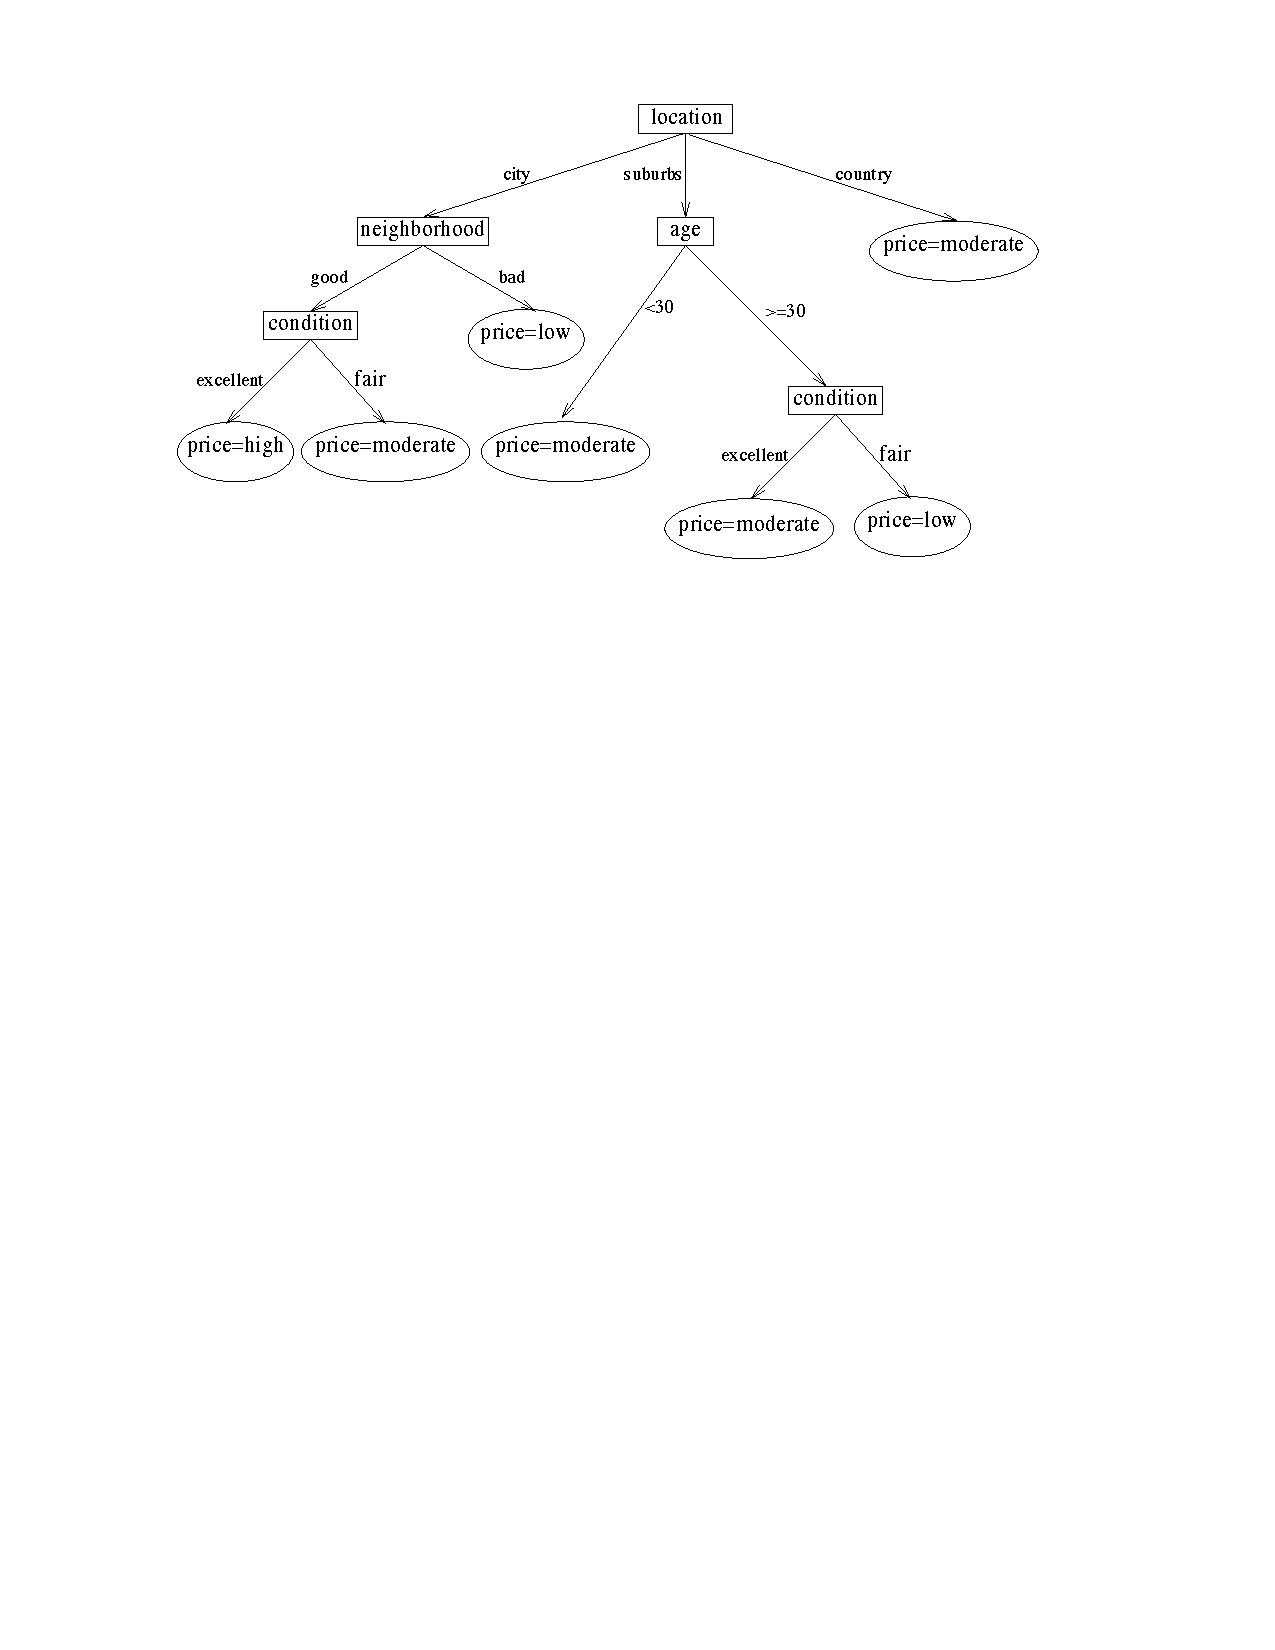
\includegraphics[width=0.86\textwidth]{dt} \caption{Example of a decision
  tree, Rectangles represent internal nodes and ovals represent leaf nodes
(possible solution)\cite{KER:70953}} \label{fig:dtree} \end{center} \end{figure}

Decision tree classifiers can be used in large datasets with high dimensional
data and still be fast and easy to understand its result. One of its' main
advantages due to its white box model of learning, is that at anytime it is
possible to understand the reason behind each and every result. In addition to
that, decision tree classifiers are very robust and require no prior knowledge
of the domain or parameter settings.

On the other hand, the problem of learning an optimal decision tree is
NP-Complete \cite{Hyafil197615}. Therefore, in practical applications of
decision tree learning algorithms, some heuristics need to be used, usually a
greedy algorithm, which can lead to local optimal decisions being made for each
node. The utilization of such algorithms cannot guarantee the global optimal
solution to the problem. There are many algorithms that implement the decision
tree principles, such as ID3, C5.0 and CART.

\subsubsection{Random Forests}

Random Forests \cite{raey} are an ensemble learning method for classification
and regression, that operates by generating a given number of decision trees
from a randomly selected with replacement subset of the complete training
dataset, where the subset distribution is the same across the forest. After
that, at each node a randomly chosen subset of variables are used for the
selection of the best split. This process continues until the trees are fully
expanded. There is no pruning of the trees.

Random Forests are robust and fairly able to deal with unbalanced and missing
data on the datasets. It is easy to set up with very little configuration
parameters and it also gives good results even when the default parameters are
used. The biggest limitation of this algorithm is not being able to predict
beyond the range of the training data when used for regression, because randomly
selected inputs give better results in classification than regression
\cite{raey}.

\subsubsection{Support Vector Machines}

Support Vector Machine (SVM) is a supervised learning algorithm with great
results in pattern recognition. \cite{Cortes95support-vectornetworks} To achieve
this results, SVMs rely on spatial division of classes. The division can be made
without dimensional limit. In other words, the plane or hyperplane that
separates the classes can have any number of dimensions. In figure
~\ref{fig:svm_nonlin} we can see an example of this multidimensional spatial
division.

%\cite{citeulike:989242}
\begin{figure}[h] \begin{center} \leavevmode
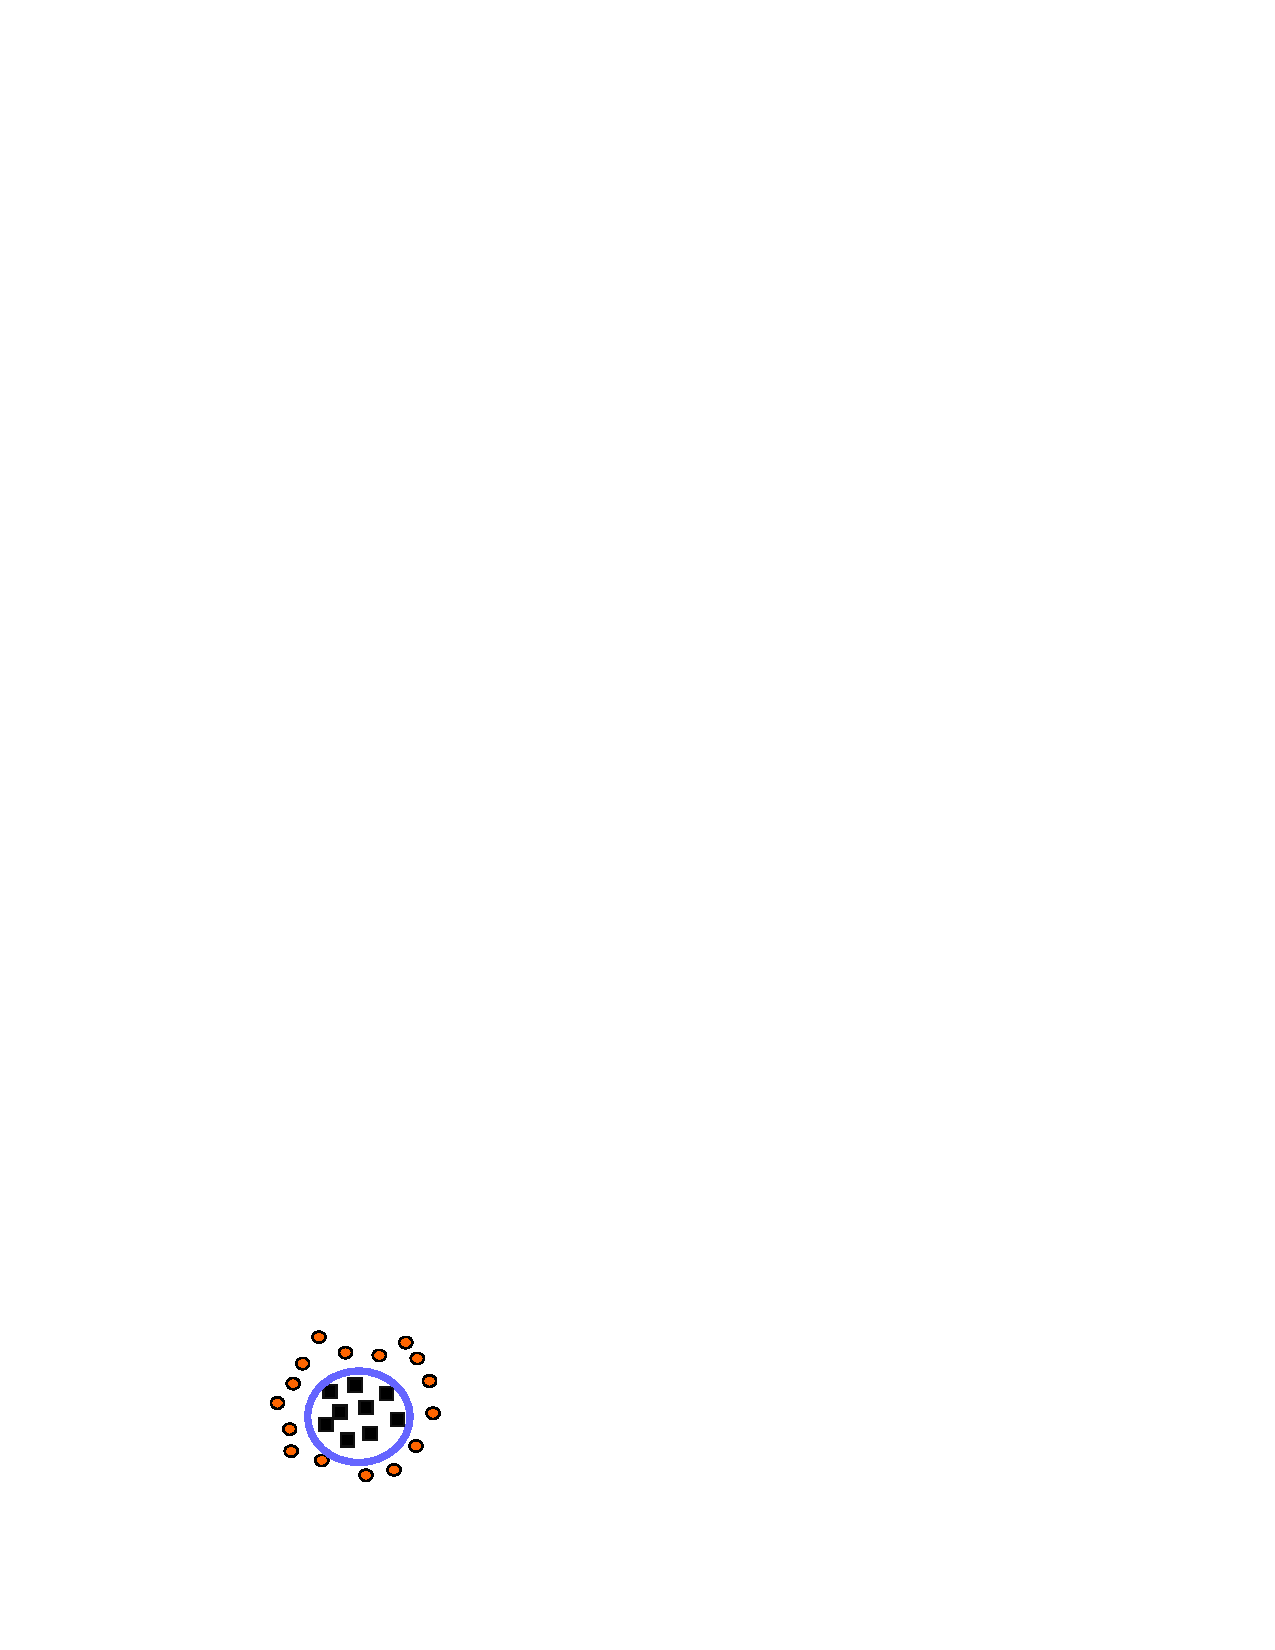
\includegraphics[width=0.66\textwidth]{svm_nl} \caption{Example of a non linear
separation (quadratic discriminant)\cite{Bennett03supportvector}}
\label{fig:svm_nonlin} \end{center} \end{figure}

However, the speed of training and testing is low, even for fastest SVMs. It is
also directly limited to two-class tasks\cite{Cortes95support-vectornetworks},
requiring to reduce multi-class tasks to binary ones. Although, some work has
been done to try to avoid decomposing the problem in multiple binary class
problems.\cite{Crammer:2002:AIM:944790.944813}

In the past few years, this method is also being used to classify internet
traffic with excellent results.\cite{Yuan2010}


\subsubsection{KNN}

The \emph{k-nearest-neighbor} algorithm is among the most simple classification
algorithms and it has been around since the 1950s \cite[p.348]{HanKam06}. KNN is
a non-parametric method which can be used in classification and regression
problems and it is mostly used in the area of pattern recognition. This
algorithm is a type of instance-based learning, or lazy learning, which means
that every computation is deferred until classification. By deferring
computation to the classification phase this algorithm is slow at classifying
instances. To classify a new instance, the algorithm has to calculate the
\emph{Euclidean distance} between the new instance and every instance in the
training set.

Since the introduction of this algorithm, some variations of it appeared to help
solving the shortcomings of \emph{kNN}.\cite{DBLP:journals/corr/abs-1007-0085}
The more notable are: \begin{itemize} \item \textbf{Clustered k nearest
      neighbor} \cite{journals/jcp/ZhouLX09} is an improved version of k-nn
      mixed with a clustering algorithm, which allow, for example, better
    performance in text classification. \item \textbf{k-d tree nearest neighbor
      (kdNN)} \cite{Sproull1991} helps to improve, in some cases, the completion
      time of the classification in logarithmic time. \item \textbf{Orthogonal
    Search Tree Nearest Neighbor} \cite{955110} greatly improves efficiency of
k-nn, especially for large datasets. \end{itemize}

\subsection{Clustering Algorithms}\label{sec:clust}

Clustering is the process of grouping similar entries/objects into different
groups, in other words, it is the method of breaking a set into various subsets
according to some metric. This groups/subsets are not known from the start and
clustering is sometimes considered the most important unsupervised learning
problem\cite{DBLP:journals/corr/abs-1205-1117}.

Clustering methods can be divided into\cite{HanKam06}: \begin{itemize} \item
      \textbf{Partitioning Methods} start with an initial number of groups, and
      reallocates iteratively the elements on the groups to
      convergence\cite{DBLP:journals/corr/abs-1205-1117}. Some examples of
      partitioning methods are based on heuristics like \emph{k-mean algorithm}
      and \emph{k-medoids algorithm}.

\item \textbf{Hierarchical Methods} work by grouping data into a tree of
  clusters\cite{HanKam06}. This methods can be further divided into two groups:
  \emph{agglomerative} (bottom-up) and \emph{divisive}
  (top-down)\cite{DBLP:journals/corr/abs-1205-1117}. At the beginning of an
  \emph{agglomerative} algorithm, each object is a cluster and these clusters
  merge with each other, to form less but larger clusters. The opposite occurs
  for \emph{divisive} algorithms. The end condition for both is a distance
  threshold.\cite{HanKam06}

\item \textbf{Density-Based Methods} were developed to find clusters with odd
  forms, relying on the premise that the clusters are located in high density
  areas that are separated from each other by low density zones \cite{HanKam06}.
  Some examples of algorithms which implement this method are \emph{DBSCAN} and
  \emph{SSN}.

\item \textbf{Grid-Based Methods} uses a multiresolution grid data structure. It
  divides the object space into a finite number of cells, that form a grid
  structure, on which all of the operations for clustering are performed. This
  approach has a fast processing time, which is typically independent from the
  number of data objects but, on other hand, dependent on the number of cells
  per dimension on the object space\cite{HanKam06}. Some examples of algorithms
  which implement the rules of this method are \emph{STING}, \emph{WaveCluster}
  and \emph{CLIQUE}.

\item \textbf{Model-Based Clustering Methods} tries to understand the
  mathematical rule behind the data, in other words, it is an ''attempt to
  optimize the fit between the given data and some mathematical model''\cite[p.
  429]{HanKam06}. This method assumes that the data was generated with some
  underlying probability. Some examples of this algorithms are
  \emph{Expectation-Maximization}, \emph{Conceptual Clustering} and \emph{Neural
  Networks}.

\end{itemize}
%\subsection{Regression Algorithms}\label{sec:regr}
\subsection{Time Series Prediction}\label{sec:tsp} One of the main problems, is
to accurately predict the volumes of the inventory. Since the data has temporal
information one possible approach is to use time series prediction to calculate
future values of time series calculated from the datasets. \\

\cite{1716527} compared three forecasting techniques \emph{Support Vector
Machines} (SVMs), \emph{Multiple Regression} (MR) and \emph{Multilayer
Perceptron} (MLP), on power production values on multiple power plants. The
\emph{MR} outperformed the other two methods on predicting those values. \\

\cite{Sabry:2007kq} compared \emph{ARIMA} with logistic regressions algorithms
to predict traffic on three Egyptian intercity roads. The average annual,
monthly and weekly daily traffic volumes were calculated using both logistic
regression and \emph{ARIMA} algorithms. They concluded that \emph{ARIMA}
outperforms the logistics regression methods in forecasting this traffic
volumes.

\subsubsection{Arima} \emph{ARIMA} also known as Box-Jenkins, is a modelling and
forecasting approach. It combines three processes, the \emph{Autoregressive}
(AR), differencing to strip off the integration (I) of the time series and
\emph{Moving Average} (MA).

Each one of this processes handle the random disturbance in its on
way.\cite{Sabry:2007kq} The \emph{AR} part of this approach is the linear
regression of the series against one or more prior values of the series. A time
series is suceptible to capture noise shocks on a noisy environment and it may
memorize this shocks for a while, the \emph{MA} term is used to capture the
outcomes of this shocks in the future.\cite{1578206} The combination of this to
terms compose the \emph{ARMA} model.

The \emph{ARMA} model assumes that the data is stationary, which is, the
statistical propreties of the data doesn't change overtime. However, this
assumption doesn't hold against most of real time series.\cite{box2013time} So,
the \emph{Integration} process has introduced in order to remove the impact of
non-stationary data by differencing.

The three processes, AR (p), I (d) and MA (q) are combined and compose the ARIMA
(p, q, d) model.

\subsection{Data Mining Tools} Today there are lots of free tools on the
internet which can help us to test and use data mining techniques. Some of the
most used will be presented bellow.

\subsubsection{Weka}

Weka\footnote{ Available at \url{http://www.cs.waikato.ac.nz/~ml/weka/}} is a
popular, open source, suite of machine learning software written in Java. It was
created at the University of Waikato, New Zealand in 1997. It has an easy to use
and comprehensive GUI with access to an enormous deck of machine learning
algorithms.

\begin{figure}[h] \begin{center} \leavevmode
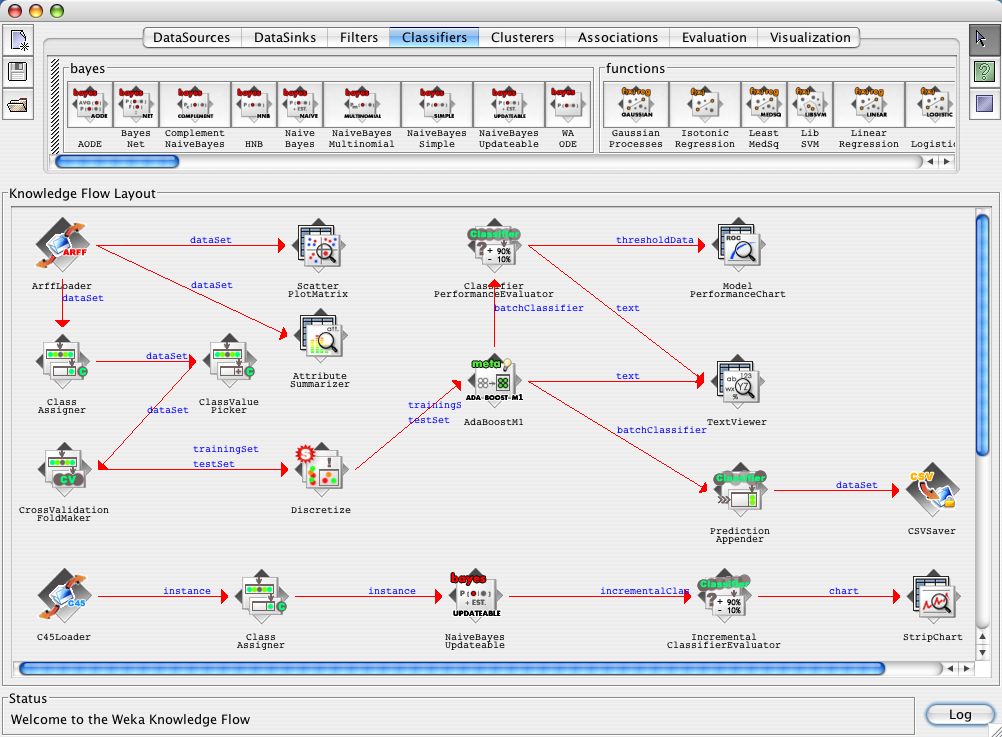
\includegraphics[width=0.66\textwidth]{wekaKF} \caption{Screenshot of Weka
\protect\footnotemark} \label{fig:RapidMiner} \end{center} \end{figure}
\footnotetext{
\url{http://www.siliconafrica.com/wp-content/themes/directorypress/thumbs//weka.png}}

\subsubsection{Apache Mahout}

Apache Mahout\footnote{ Available at \url{http://mahout.apache.org}} is an open
source machine learning library to build scalable machine learning libraries.
Its core algorithms are implemented on top of map/reduce paradigm, to help in
the scalability of the solution. Since it is easier to get a cluster of server
than an ultra high frequency CPU, and the market trend is to develop many and
multi core solution, it is always the best option for processing large
quantities of data scalable software.

According to their website, \emph{Mahout} has: \begin{itemize}

\item User and Item based recommenders \item Matrix factorization based
recommenders \item K-Means, Fuzzy K-Means clustering \item Latent Dirichlet
Allocation \item Singular value decomposition \item Logistic regression based
classifier \item Complementary Naive Bayes classifier \item Random forest
decision tree based classifier \item High performance java collections
(previously colt collections) \item  A vibrant community

\end{itemize}

\subsubsection{RapidMiner}

Rapid Miner\footnote{ Available at \url{http://www.rapidminer.com/}} is a
complete solution for data mining problems. It is available in a form of a
standalone GUI application. \begin{figure}[h] \begin{center} \leavevmode
  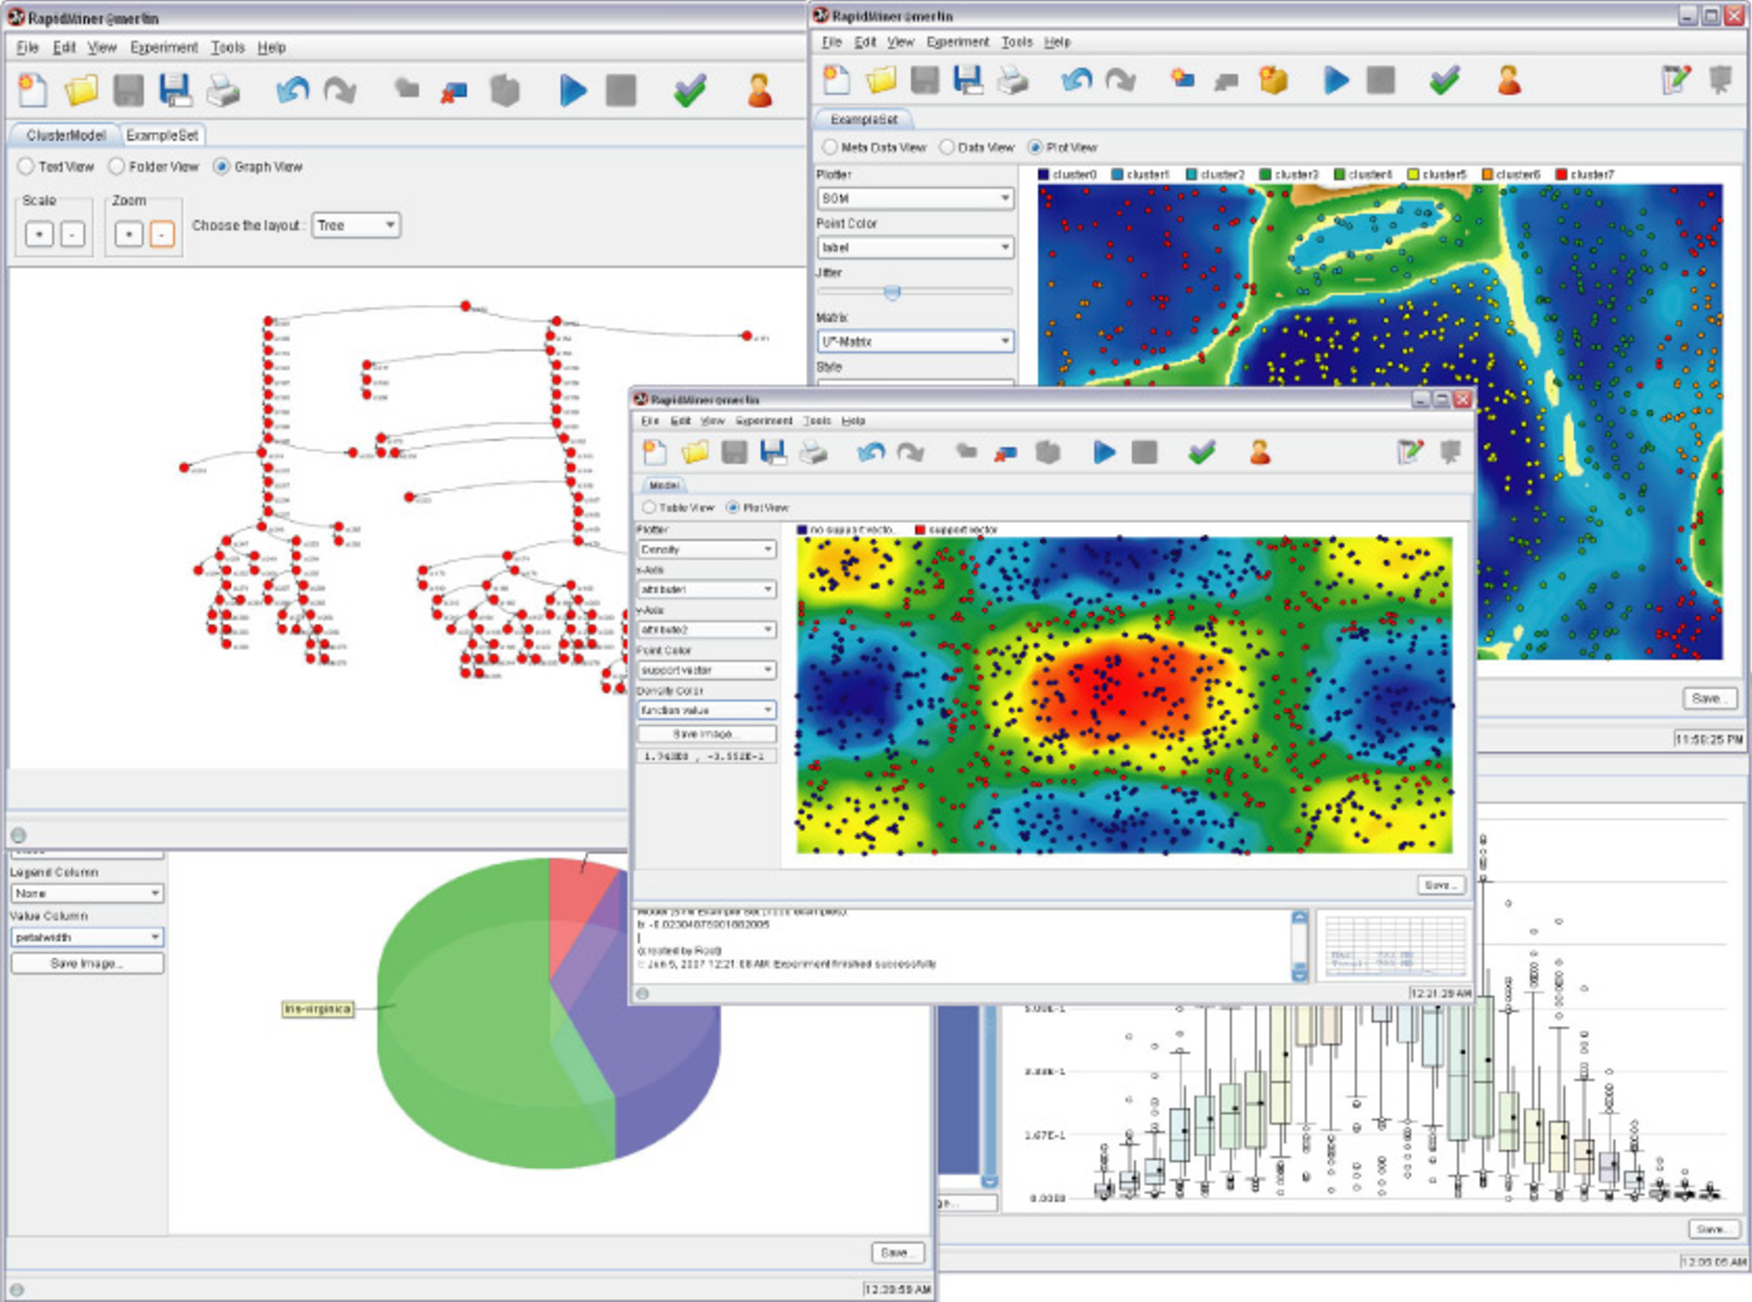
\includegraphics[width=0.66\textwidth]{rapidminer} \caption{Screenshot of
RapidMiner \protect\footnotemark} \label{fig:RapidMiner} \end{center}
\end{figure} \footnotetext{
\url{http://mloss.org/media/screenshot_archive/rapidminer_collection.jpg}}
Although it is a commercial product, there is also a free tier, and the core and
earliest versions are open source. This application is one of the main players
of this market and it is easily expandable through plug-ins available online.

\subsubsection{R Language} R\footnote{ Available at
\url{http://www.r-project.org}} is a free programming language and software
environment for graphics generation and statistical computing. Developed by Ross
Ihaka and Robert Gentleman at the University of Auckland, New Zealand, in 1993
\cite{Ihaka98r:past}, it is still in active development and greatly used by
statistics and data miners.

R is an implementation of S, the statistics programming language, and it uses
some characteristics inspired on Scheme. R is a GNU tool, so it is completely
free. There are wrappers to almost every language which can be used to access R
variables from other programming languages.

\section{Model Evaluation Procedures and Measures}

To verify if a created model is valid it is necessary an additional step to
validate the data. This step can be divided into evaluation procedures, which
normally consists of dividing the original dataset into training and testing
subsets, and evaluation measures in order to assess the quality of our model.

\subsection{Model Evaluation Procedures} \subsubsection{Cross-Validation}

This model consists of dividing the dataset in parts
\cite{Witten:2005:DMP:1205860} . Some of these parts will be used to train the
model and other parts will only be used in the validation part, so that we can
assess if the model is able to generalize the result or not. 

\paragraph{Sliding Window}

This procedure selects its training data and validation data maintaining the
chronological order of the data set\cite{Bensch_self-learningprediction}.

\begin{figure}[!h] \begin{center} \leavevmode
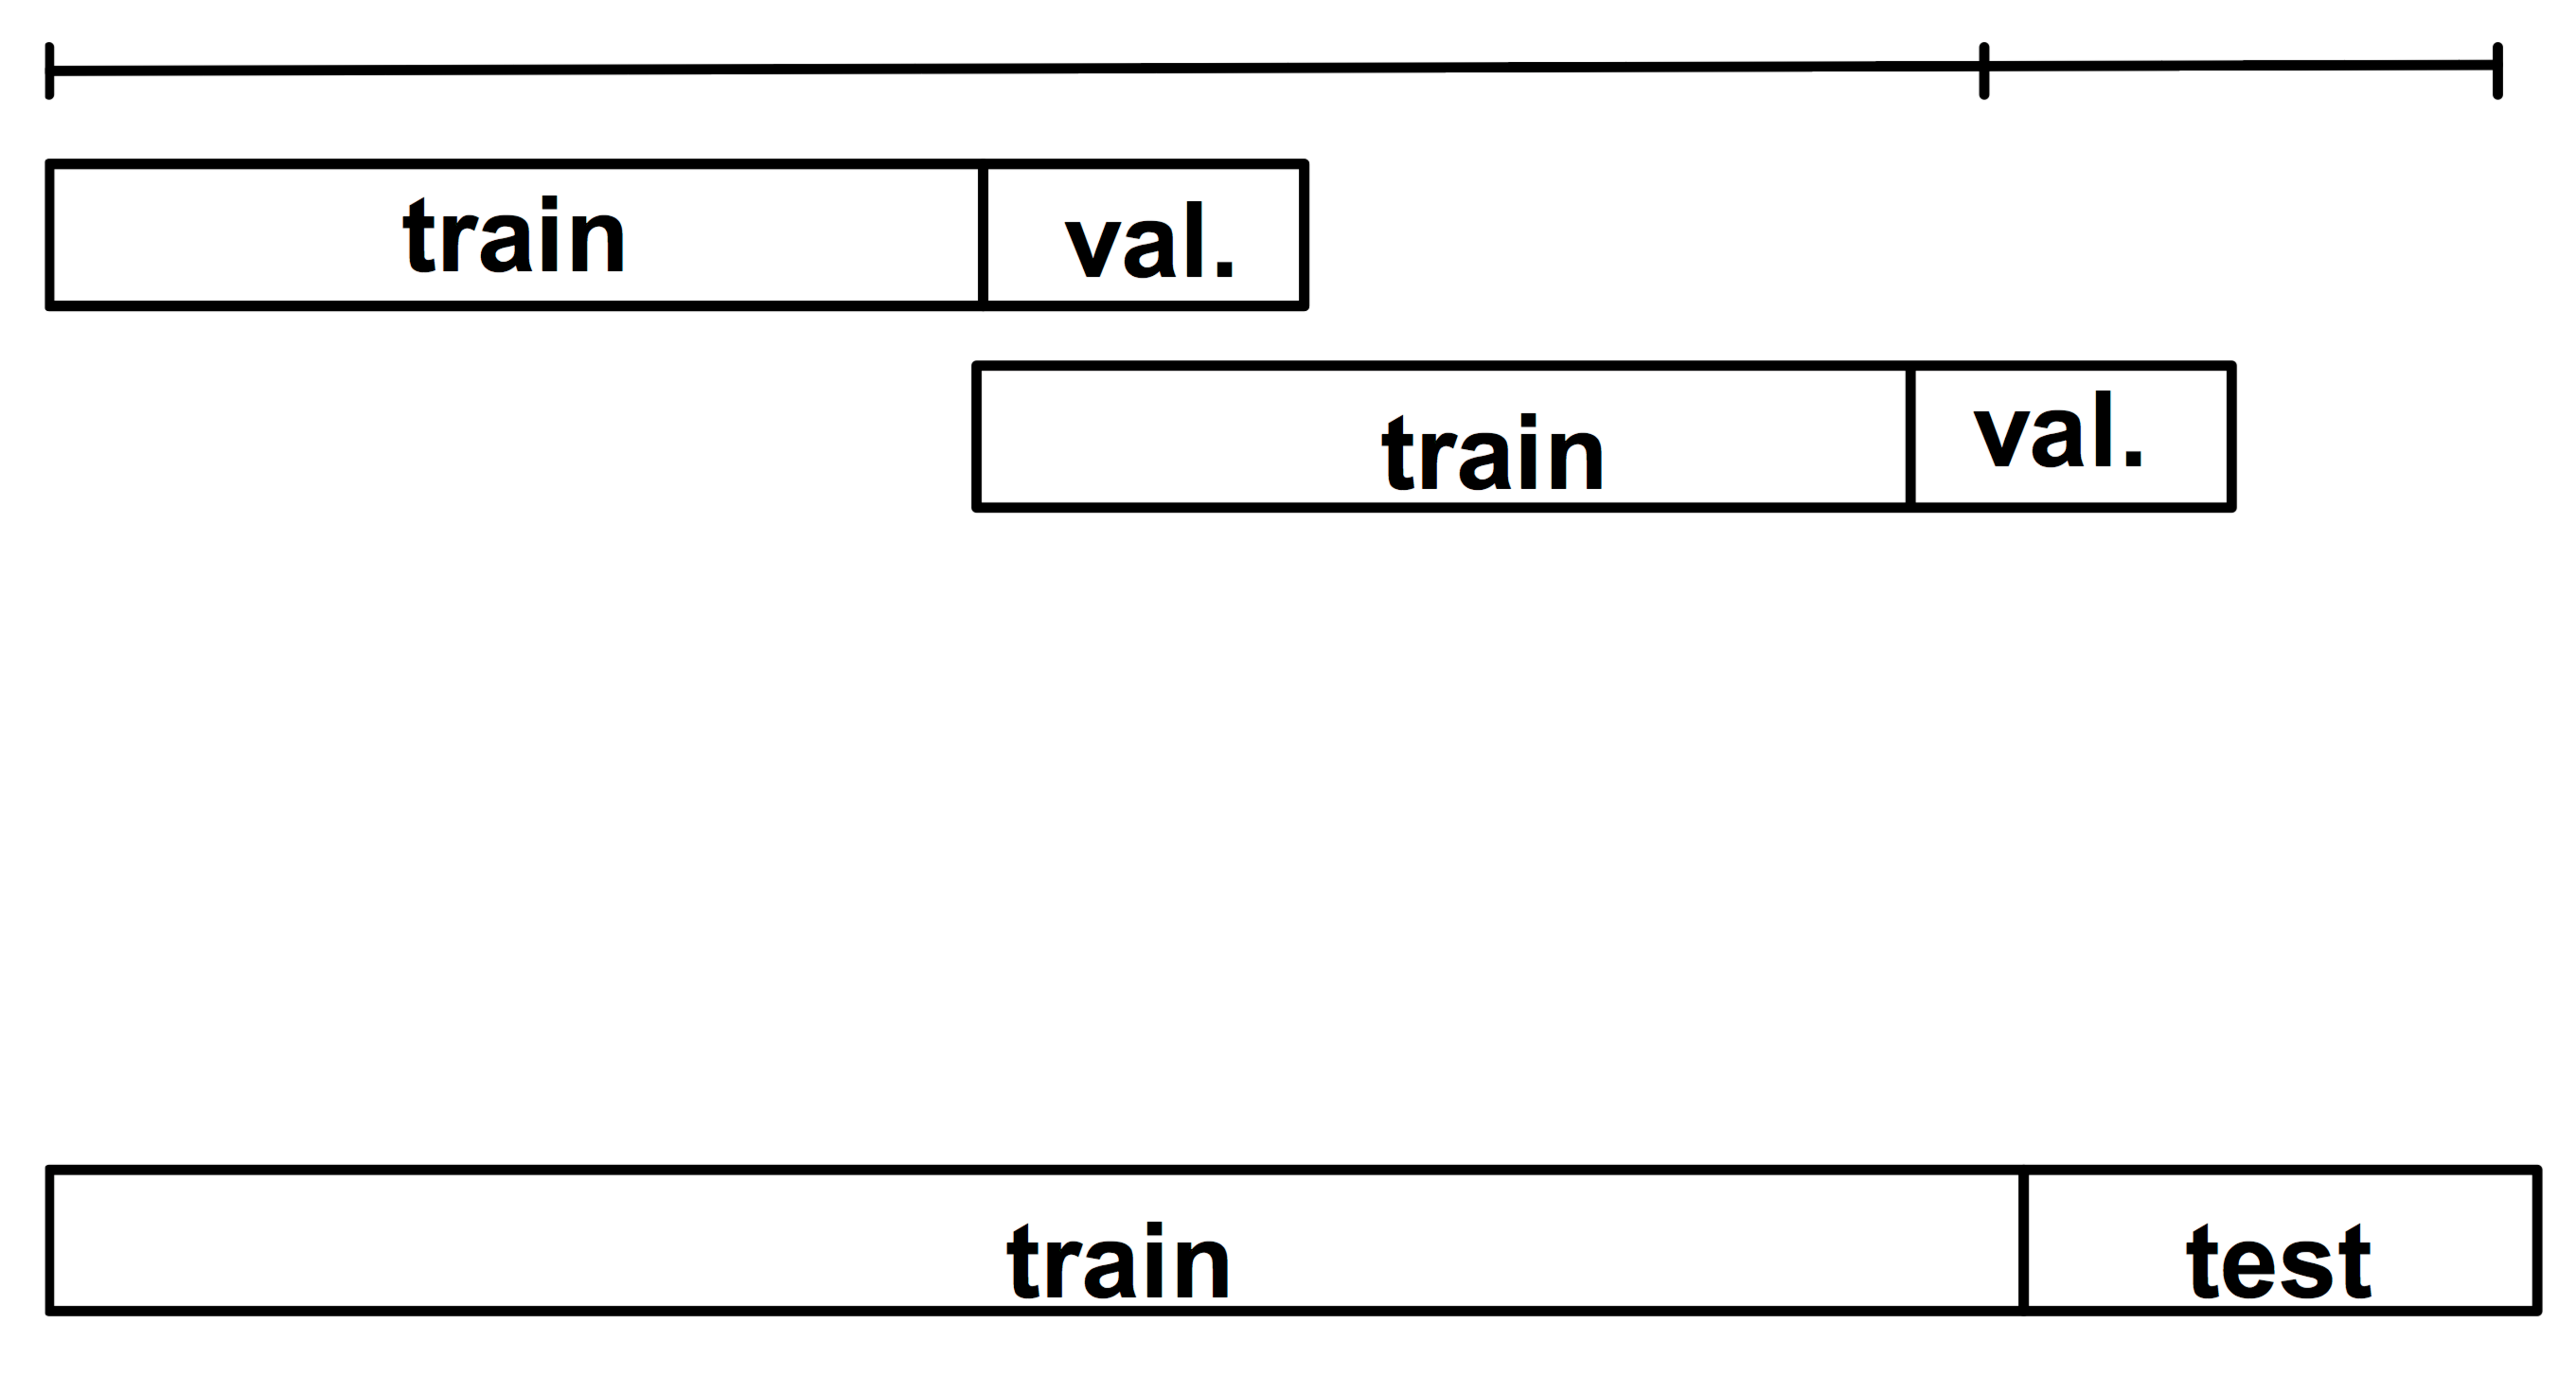
\includegraphics[width=0.66\textwidth]{swin} \caption{Sliding window validation}
\label{fig:swin} \end{center} \end{figure} \FloatBarrier

In figure~\ref{fig:swin}, it possible to see that the validation data happens
after the training data in a temporal point of view.

\subsection{Model Evaluation Methods}

\subsubsection{Precision}

Precision is a metric to identify the fraction of positives that are correctly
classified as so. In other words, using this measure, we can identify how
relevant the results given by the algorithm are (the more higher the value, the
more relevant the results are). The equation to calculate precision is presented
next:

\begin{center} \Large \begin{math} Precision = \frac{\text{true
positives}}{\text{true positives + false positives}} \end{math} \normalsize
\end{center}


\subsubsection{Recall}

This measure represents the part of actual positive results in the dataset that
were identified as such. In other words, recall is the fraction of positive
objects that were correctly identified by the algorithm from all the positive
objects in the dataset. This metric is calculated using the following
expression:

\begin{center} \Large \begin{math} Recall = \frac{\text{true
positives}}{\text{true positives + false negatives}} \end{math} \normalsize
\end{center}

\subsubsection{Accuracy}

Accuracy represents the percentage of results that are actually correct. This
measure can be calculated as follows:

\begin{center} \Large \begin{math} Accuracy = \frac{\text{true positives + true
negatives}}{\text{true positives + false positives + true negatives + false
negatives}} \end{math} \normalsize \end{center}


\subsubsection{F-Measure}

F-Measure or F-Score or F\begin{math}_1 \end{math} measures the test accuracy
  relying in both recall and precision. The best value of this function is 1 and
  the worst is 0. F-Measure is the harmonic mean of the precision and recall and
  can be defined as it follows:

\begin{center} \Large \begin{math} F_1 = 2 *
\frac{precision*recall}{precision+recall} \end{math} \normalsize \end{center}

The reason behind the utilization of the harmonic mean instead of the arithmetic
mean is given due to a more intuitive result \cite{sasaki2007truth}. \\

\subsection{Time Series Forecast Accuracy Evaluation}

There are various methods of accuracy evaluation for time series. In
\cite{Hyndman2006679} a large scale comparison of various methods such as
\emph{Mean Absolute Percentage Error} (MAPE), \emph{Median Absolute Percentage
Error} (MdAPE), \emph{Symmetric Mean Absolute Percentage Error} (sMAPE),
\emph{Symmetric Median Absolute Percentage Error} (sMdAPE), \emph{Median
Relative Absolute Error} (MdRAE), \emph{Geometric Mean Relative Absolute
Error} (GMRAE) and \emph{Mean Absolute Scaled Error} (MASE). This publication
recommends the usage of \emph{MASE} in favor of the others because the
situations where this measure gives undefined or infinite results are almost
irrelevant.

\subsubsection{Overview}
\begin{table}[h] \begin{center} \leavevmode
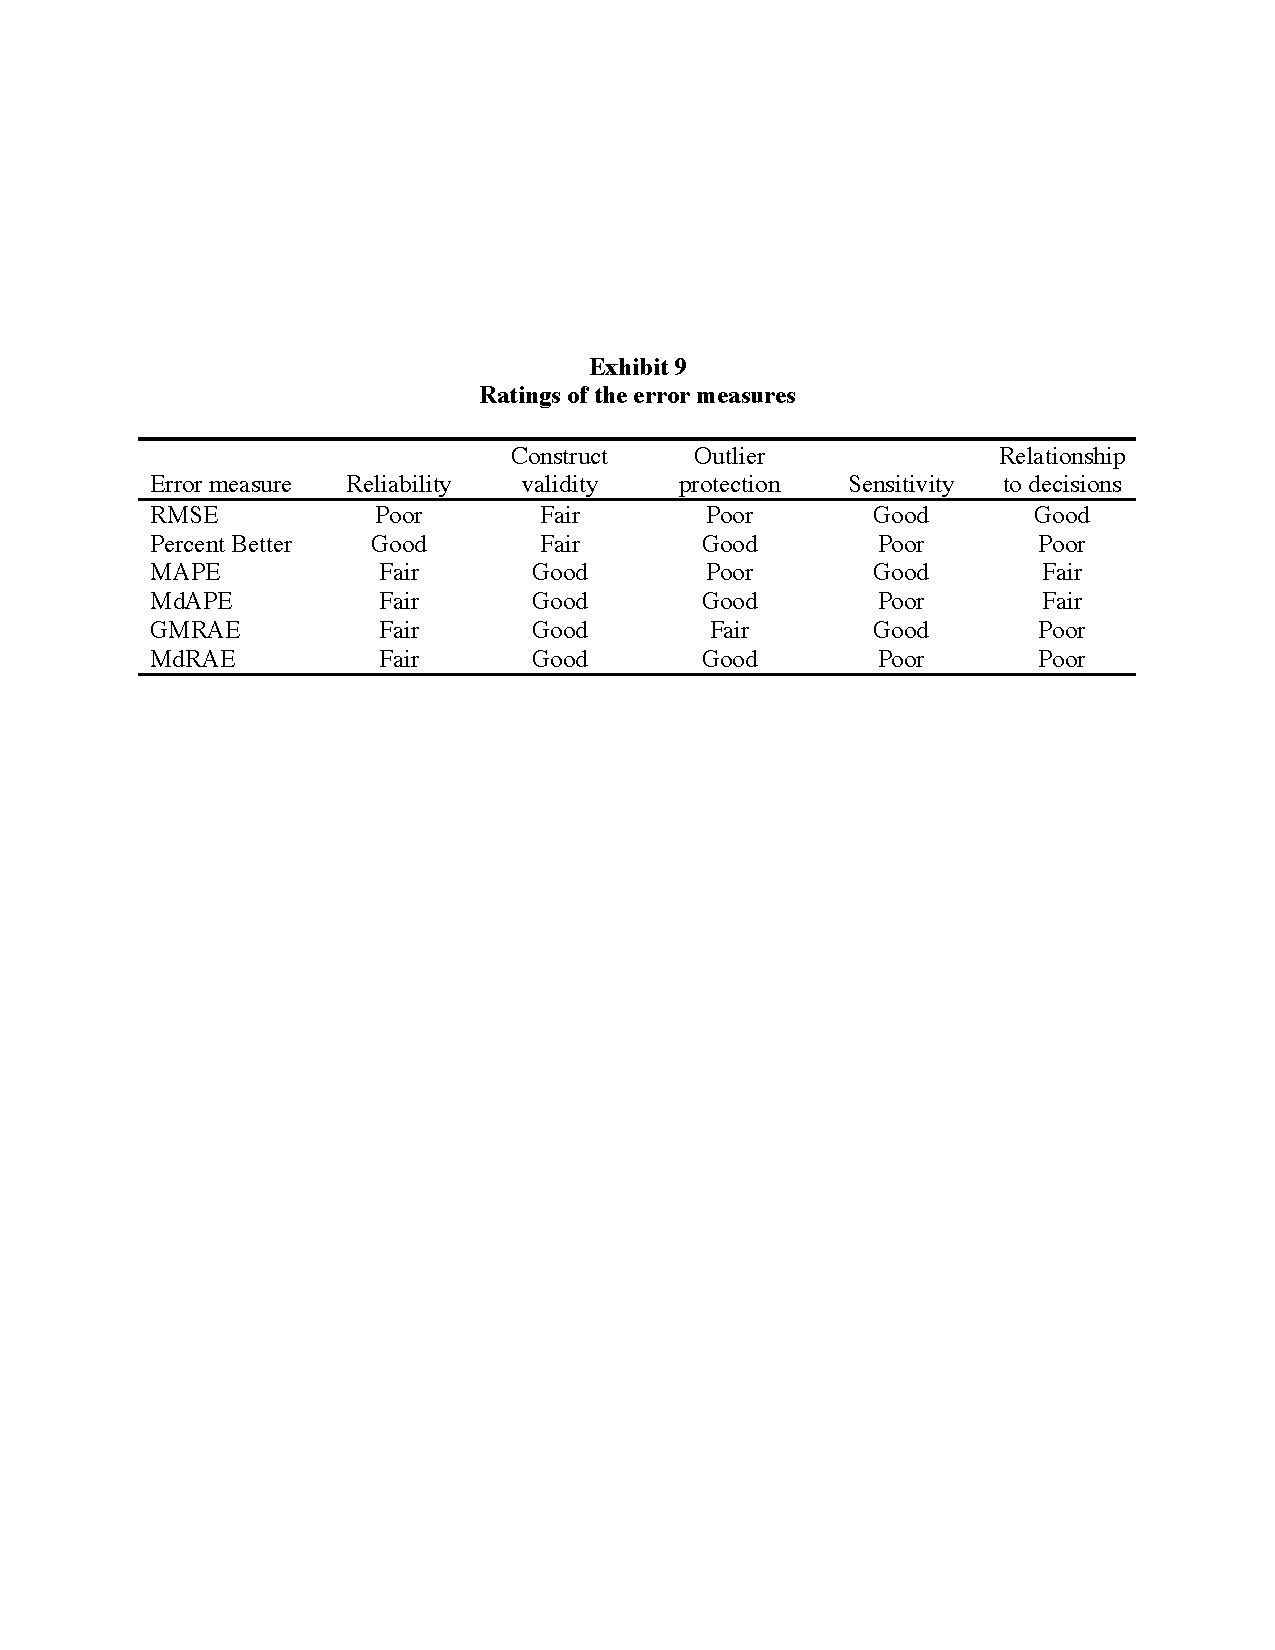
\includegraphics[width=0.96\textwidth]{tsp_comparison} \caption{Guidelines for
selecting error measures \cite{Armstrong199269} } \label{fig:ts_error_selection}
\end{center} \end{table}

In the Table~\ref{fig:ts_error_selection} the author tries to make easier to
choose between the methods described forward.

\subsubsection{Scale-dependent measures}

These accuracy measures are commonly used whose scale depends on the scale of
the data. So these methods shall only be used when comparing different methods
applied to the same data set, and shall never be used when comparing across
different data sets whose have different scales.
\\

Forecast error can be defined as \begin{math} e_t = Y_t - F_t \end{math}, let
\emph{Yt} denote real observation at time \emph{t} and \emph{Ft} being the
forecast value.
\begin{itemize}
  \item \textbf{Mean Squared Error} (MSE) = mean(\begin{math} e_t^2 \end{math})
    \item \textbf{Root Mean Square Error} (RMSE) = \begin{math}
      \sqrt{MSE}\end{math}
  \item \textbf{Mean Absolute Error} (MAE) = mean(\begin{math}
      \left|e_t\right|\end{math})
  \item \textbf{Median Absolute Error} (MdAE) = median(\begin{math}
      \left|e_t\right|\end{math})

\end{itemize}

Some authors \cite{Armstrong:2001fj} recommend the usage of \emph{MAE} and
\emph{MdAE} instead of \emph{MSE} and \emph{RMSE} since the last are more
susceptible to outliers than the first ones.


\subsubsection{Measures based on percentage errors}

The percentage error have the advantage of being scale independent thus can be
used to compare forecast performance across different datasets.

The percentage error is given by \begin{math} p_t = 100 * \frac{e_t}{Y_t}
\end{math}.


The most common measures are:
\begin{itemize}
  \item \textbf{Mean Absolute Percentage Error} (MAPE) = mean(\begin{math}
      \left|p_t\right|\end{math})
    \item \textbf{Median Absolute Percentage Error} (MdAPE) = median(\begin{math}
      \left|p_t\right|\end{math})
    \item \textbf{Root Mean Square Percentage Error} (RMSPE) = \begin{math}\sqrt{mean(
      p_t^2)}\end{math}
    \item \textbf{Root Median Square Percentage Error} (RMdSPE) = \begin{math}\sqrt{median(
      p_t^2)}\end{math}
\end{itemize}

The major drawback of these measures is for \begin{math} Y_t = 0 \end{math} the
value is infinite or undefined for any \begin{math} t \end{math} and have a
very skewed distribution when compared when any value of \begin{math} Y_t
\end{math} is close to 0.
The \emph{MAPE} and \emph{MdAPE} also have the disadvantage of put a heavier
penalty on positive errors than on negative errors. This observation lead to the
use of another percentage error based measures. The "symmetric" measures
\cite{RePEc:eee:intfor:v:9:y:1993:i:4:p:527-529}:
\begin{itemize}
  \item \textbf{Symmetric Mean Absolute Percentage Error} (sMAPE) = mean(\begin{math}
      200 * \frac{\left| Y_t - F_t \right|}{Y_t + F_t}\end{math})
    \item \textbf{Symmetric Median Absolute Percentage Error} (sMdAPE) = median(\begin{math}
      200 * \frac{\left| Y_t - F_t \right|}{Y_t + F_t}\end{math})
\end{itemize}

In case of the time series used have negative values, there are the risk of
divide by zero. Furthermore these measures also are reported as not as
"symmetric" as the name suggests. Mostly because the penalty is heavier when the
forecasts are low when compared with when the forecasts are high. \cite{Goodwin1999405}

\subsubsection{Measures based on relative errors}

Another approach for scaling is to divide each error by the error obtained by
another standard method of forecasting. So relative error is defined by
\begin{math} r_t = \frac{e_t}{e_t^*} \end{math}, where \begin{math} e_t^*
\end{math} is the forecast error obtained from the benchmark method. Usually
this baseline method is the random walk where \begin{math}F_t\end{math} is equal
to the value of the last observation.
So the measures can be defined:
\begin{itemize}
  \item \textbf{Mean Relative Absolute Error} (MRAE) =
  mean(\begin{math}\left|r_t\right|\end{math})
  \item \textbf{Median Relative Absolute Error} (MdRAE) =
  median(\begin{math}\left|r_t\right|\end{math})
  \item \textbf{Geometric Mean Relative Absolute Error} (GMRAE) =
  gmean(\begin{math}\left|r_t\right|\end{math})
\end{itemize}

\subsubsection{Relative measures}

As a substitute of the usage of relative error is the usage of relative
measures. One example, is calculate the \emph{MAE} of the baseline
(\begin{math}MAE_b\end{math}) and use the result to calculate the relative
\emph{MAE} defined by:
\\

\begin{center}
\Large
\begin{math}
  RelMAE = \frac{MAE}{MAE_b}
\end{math}
\normalsize
\end{center}

Similar approaches can be applied to other measures described before.
The main advantages of these approaches is their interpretability, since if
\emph{RelMAE}<1 then the proposed method is better than the baseline and when
the \emph{RelMAE}>1 then the proposed method is worst than the baseline.
A related approach is to use the percentage of forecasts which a given model is better than
the baseline method.\cite{Armstrong199269} Can be defined as:
\\

\Large
\begin{align*}
 PB_m=\frac{\sum\limits_{t=1}^n j_t}{n}*100\\ \text{where }j_t =
 \begin{cases}\text{1 if }e_{t,m} < e_{t,b}\\ \text{0 otherwise }\end{cases}
\end{align*}
\normalsize
\\

This approach describes a method \emph{m} with a \emph{PB} score relative to the
baseline.

\subsubsection{Scaled errors}

The author of the paper \cite{Hyndman2006679} propose this approach to address
the situations where more traditional scaled accuracy measures fail (as
described before). So the scaled error is described as it follows:

\begin{center}
\Large
\begin{math}
  q_t = \frac{e_t}{\frac{1}{n-1}*\sum\limits_{i=2}^n\left|Y_i - Y_{i-1}\right|}
\end{math}
\normalsize
\end{center}

A scaled error is less than one if the method forecast is better than the
average one-step na\"{i}ve forecast computed in sample. Otherwise, if the error
is greater than one the method is worst than the na\"{i}ve approach.
So the \textbf{Mean Absolute Scaled Error} (MASE) is defined simply by

\begin{center}
\Large
\begin{math}
  MASE = mean(\left|qt\right|)
\end{math}
\normalsize
\end{center}

In a similar manner the results of \emph{MASE} for a method, if less than one
the method is better than the na\"{i}ve approach and worse otherwise.
Related methods such as \emph{Root Mean Squared Scaled Error} (RMSSE) and
\emph{Median Absolute Scaled Error} (MdASE) can be defined in a similar manner.
The only situation where this method falls short is when the historical data has
always the same value since the denominator would be 0 and make the result of
\emph{MASE} infinite or undefined.


\section{Web Usage Mining}\label{sec:network}

\nocite{UjwalaPatil}

The main area which this project focus on is the utilization of ad requests logs
to predict future requests of the users. This is analogous to work which have
been done in the area of user future requests prediction. Next, it will be done
a little overview of what has been studying in the area of web usage data mining
in the past years, in order to identify possible approaches to solve the problem
of this thesis.

\paragraph{}

In the area of pre-fetching web pages \cite{Nanopoulos01effectiveprediction}, it
has been proposed a new algorithm, WM\begin{math}_0\end{math}, which takes into
  account the order between accesses and other specificities of the area. This
  algorithm gets good results for accuracy even when compared to other methods
  like \emph{Prediction-by-Partial-Match} (PPM) and \emph{Dependency Graph}
  (DG).

\paragraph{}

In another paper \cite{Gery:2003:EWU:956699.956716}, three approaches to data
mine from web logs are proposed. \textbf{Association Rule} (AR) is based on
association rule learning which is a very popular data mining family of
algorithms to find relationships between variables. The problem of finding web
pages together in a web log is similar to that problem. \textbf{Frequent
Sequences} (FS), is a technique that tries to find time ordered sequences of
URLs that have been followed by past users. \textbf{Frequent Generalized
Sequences} (FGS) involves the utilization of a generalized sequence, which is a
sequence that allows wild cards in order to represent a user flow of navigation
in a more flexible way. Some tests have been made by the author
\cite{Gery:2003:EWU:956699.956716} to test the performance of this three methods
using real web logs. According to the results given by FS, FS has better
accuracy than AR and FGS.

\paragraph{}

In another paper, other author proposes a model that preserves sequentiality of
the clicks \cite{Frias-Martinez2003}. The rules maintain the sequence of the
click stream between the antecedent and the consequent, to maintain
sequentiality. This model also introduces the concept of temporality, which is
reflected by the distance between the consequent and antecedent by number of
clicks to go from one to the other. This rule is very important because it
allows not only to find which page is  going to be accessed but also when will
it be accessed. The proposed model, \textbf{Customizable Sequential Behavior
Model}, can be adapted depending on the characteristics of the server, in order
to capture the behavior of the users more accurately.

\paragraph{}

There is another approach that relies on the sequentially of the clicks
\cite{Jan:2007:WUB:1353862.1353874}. This method uses the prefix set of web
pages (pages that the user had already visited) to predict a postfix set (next
pages that the user will visit). To select this pages, the algorithm uses a
confidence threshold to select the pages to the postfix set from historical
data.


\paragraph{}

An approach based on the \textbf{Longest Common Subsequence} (LCS)
\cite{4631852} has also been used in web usage mining. In this case, the author
proposes a two part architecture: an offline part where knowledge is extracted
from the historical data and an online part where this knowledge is used to
predict the next visits of the user. The prediction is done in the online part
by appending the last request from the user to the history and using LCS. This
architecture is implemented in \textbf{WebPum} \cite{Jalali20106201} by the same
authors and improves the accuracy by a little margin from the previous method,
SUGGEST 3.0 \cite{1410804}, in the field of next page recommendations.

\paragraph{}

In other paper a method combining Markov model based sequential pattern mining
with clustering is proposed \cite{Anitha_anew}. This combination gets about 12\%
more accuracy when compared with the traditional Markov model. The proposed
models combine great accuracy from high order Markov Models with less space
complexity from low order Markov models.

\subsection{Web Usage Mining applied to Online Advertising}

Data mining is also being used to predict the response of an user to an online
ad\cite{chapelle2013simple}. Their main objective is to develop a framework that
can predict the result of an user clicking in an advertising, based on the
history that they have. The proposed framework uses Maximum
Entropy\cite{Nigam99usingmaximum} because it is easy to implement, can be
parallelized and scaled with respect to the number of features. It is easy to
include model updates in this method. In this paper, they add a two-phase
feature selection algorithm, to increase the automation and reduce the need of
domain expertise (a generalized mutual information method to select the feature
groups to be included and a feature hashing to have the ability of controlling
the size of the models). To their experiments, the authors used logs with the
same parameters as the datasets that will be used on this project.

In another approach to the same problem are introduced improvements in the
context of traditional supervised learning based on FTRL-proximal online
learning algorithm \cite{McMahan:2013:ACP:2487575.2488200}. This paper also
explores ways to save memory during the prediction, using filters to select
features to be included in the model, such as \emph{Poisson Inclusion} and
\emph{Bloom Filter Inclusion}, and they concluded that the method which allows
better savings, without loosing much prediction accuracy, is \emph{Bloom Filter
Inclusion}. To solve the memory problem they also tested encoding values with
fewer bits and other techniques.

In yet another paper about CTR(Click-Through-Rate) prediction
\cite{Tagami:2013:CPC:2501040.2501978}, a two stage approach is used, the first
stage being the construction of a ranking model with the clicked ad requests and
then a sigmoid function converting the value of the ranking model into CTR. The
method proposed achieves better results in terms of AUC, MSE and LogLoss when
compared to: L2-loss linear SVM, logistic regression with only the clicked ad
requests and logistic regression with all the ad requests.

In the area of forecasting ad impressions, a Bayes network was used to capture
inter-dependencies between the query traffic features and the competitors in the
auction\cite{nath2013ad}. This method is used to forecast the number of
impressions of the ad to a certain keyword based on the bid that is done. Their
method, Generative Model based Ad Impression Forecasting Method, get better
results in terms of accuracy when compared to Normalized Bid Model. 
%\subsection{Instance-based regression algorithms}\label{sec:instance}

\chapter{Problem Description}\label{chap:chap3}

\section*{}

The online advertising market is huge and its size has been increasing in money,
campaigns and users. Both platforms that sell and buy space for ad placement
want to understand what is their value and more important, what will be their
value in the future. In both cases this value is mostly constrain by campaigns
and users that are target for their campaigns.

Our goal is to forecast the availability of the users in the future so we can
simulate the value of future campaigns over them.

The main problem is to predict how the future will be.
Can came from many sources

\section{Forecast Inventory Statistics}

\section{Agnostic input data processing}

\section{Objectives}


\chapter{Approach}\label{chap:chap4}

\section*{}

This chapter describes the developed approach during the course of this
dissertation. First we describe its high level architecture, and then we move on
to describe each of the main phases that comprise it. For each phase, we
describe the phase both at a general level and its materialization (its main
goal, the most important variables, constraints, and methods). 

Finally, we describe the experimental setup of the approach, and the setup for
each component, and introduce the next chapter.

\section{High-level Architecture}

\begin{figure}[h] \begin{center} \leavevmode
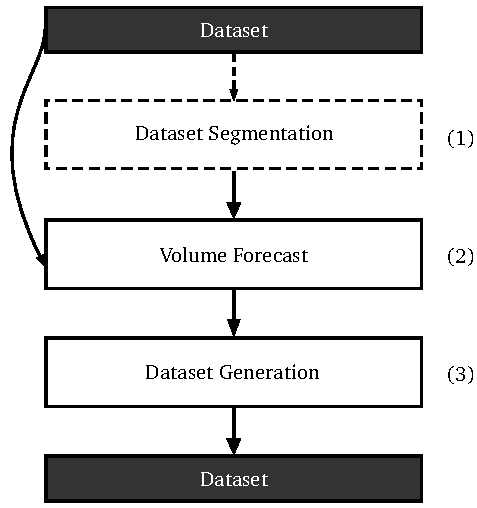
\includegraphics[]{high_level} \caption{ High level overview
of the approach } \label{fig:highlevel_arch} \end{center} \end{figure}

As the figure~\ref{fig:highlevel_arch} makes clear, the goal of the
proposed approach is to use a dataset containing logs of the web
activity from an online advertising related network and use this information 
to generate a possible future web activity logs on the same network. In such a way, that the
tendencies and the data coherency is preserved.

This approach can be divided three main phases: \emph{segmentation},
which its main purpose is divide the dataset in smaller and more predictable
datasets, in order to improve the results obtained after the second phase, mostly when there
are large quantities of data available.

The second phase is where the \emph{forecast of the volumes} that characterize the traffic on
the network are done, using time series prediction method.

The third an last phase of the process, the more complex one, is where the volumes
generated from the phase two combined with the data provided by the original
dataset are used to \emph{generate a dataset} that represent a possible future of the
web activity on the target network.

\section{Architecture for Web Activity Forecasting and Synthesising}

\subsection{Data Segmentation}\label{subsec:seg}

\begin{figure}[h] \begin{center} \leavevmode
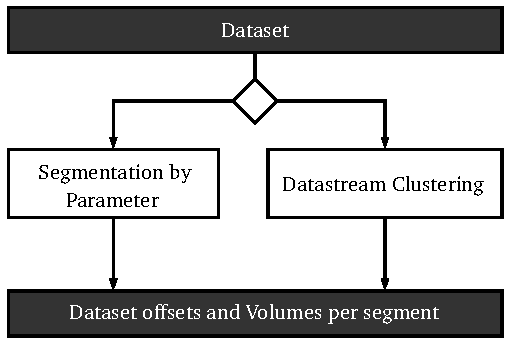
\includegraphics[]{segmentation} \caption{ High level overview
of Data Segmentation} \label{fig:segmentation_arch} \end{center} \end{figure}

The \emph{Data Segmentation} phase was designed in order to achieve better
results in the following phases. 

In order to get better results in the second phase (Volumes Forecast) the dataset needs to possess
certain characteristics that improve its predictability, or in other words, it
needs to have recurring trends and /or patterns.
One way of getting results is by splitting data by parameters known to have an
effect on traffic seasonality (for example the website that is being accessed).

As shown on figure~\ref{fig:segmentation_arch} the method described before was
one of the approaches chosen to achieve a more predictable time series.
This method allows clustering of the dataset via a selected parameter, which
returns \emph{impression clusters} in which all members of a cluster share the
same value in the parameter. This method requires great knowledge about the
available impressions to be successful.

The other approach that was implemented on this phase is a simplified and
striped down version of a \emph{data stream clustering} algorithm. This
algorithm is distance based, and since the structure of the datasets used on
this thesis are not guaranteed, the distance measure used is na\"{i}ve. The
distance between impressions can be described as:

\begin{center}
\begin{equation*}
  distance_{x,y}= \sum\limits_{i=0}^n d_i
\end{equation*}
\begin{equation*}
\text{where } d_i = \begin{cases} \text{1 if } x_i = y_x\\
\text{0 otherwise}\end{cases} \text{ and x, y are two impressions from the
dataset}
\end{equation*}
\end{center}

\begin{algorithm}
  \LinesNumbered
  \SetNlSty{texttt}{(}{)}
  \KwData{$lines$, all impressions available on the dataset; $threshold$,
  maximum distance to be considered member of a certain cluster.}
  \KwResult{A list of clusters, each one characterized by the $centroid$ and a list of
  offsets representing the position of each impression on the dataset.}
  \BlankLine

  \Repeat{no more impressions}{
    compare each impression with the existing list of clusters\;
    \eIf{ $dist < threshold$ }{
    add to the selected cluster\;
    }{create a new
    cluster and use the selected impression as the centroid for the new
    cluster\;}
  }
  \BlankLine

  \caption[Data stream clustering]{
    Data stream clustering simplified algorithm to aggregate the impressions by
    the parameters that they have in common.
  }
  \label{alg:pam} \end{algorithm}

This kind of algorithm was selected because, of the constraints imposed by the
problem, the most important ones are the huge volume of data this approach
needs to process, and the number and type of attributes that compose an
impression which may vary from dataset to dataset.

The huge volume of data invalidates the usage of a
dissimilarity matrices due to memory constraints, the uncertainty of the
parameters that are available also limit the quality of the distance measure,
since it assumes that every parameter has the same weight as the others.

This family of clustering algorithms has some known limitations, for example, the
order in which the dataset is read directly influences the outcome of the
algorithm. There is also a problem with the centroids, since they are represented
by the attributes of the impression that originated that particular centroid,
and as such are never updated,
when a new impression has a distance lower than the threshold when compared with
a certain centroid, it is not assured that the respective cluster is the most
similar to the new impression. To address that possible issue the possibility of
search over all available centroids and select the one with the smallest distance
available.

\subsection{Volume Forecasting}\label{subsec:volume_forecast}

\begin{figure}[h] \begin{center} \leavevmode
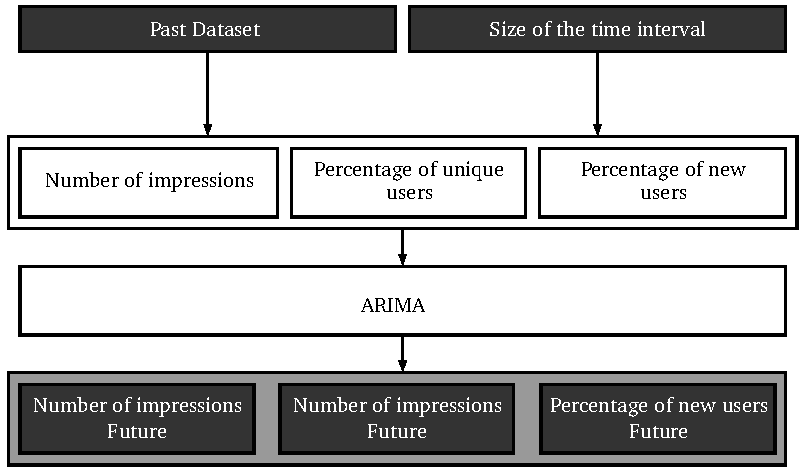
\includegraphics[]{forecast_volumes_arch} \caption{ High level overview
of Data Segmentation} \label{fig:forecast_volumes_arch} \end{center} \end{figure}

One way to describe the impressions is by representing how many happen during a
certain amount of time. So the impressions in the past can be described as time
series of volume of impressions, composed by uniformly spaced time intervals. 

So to predict how many impressions will happen in the future \emph{time series
analyses} techniques can be used. 

Since the volume of impressions doesn't allow to fully characterize the future
we need to use more time series of different variables which can provide more
 information about each epoch.

The approach here described involves the usage of three time series, one for the
number of impressions, other for the percentage unique users and a last one for
the percentage of unique users that had never appeared in the past.

\paragraph{Number of impressions}
is number of entries on the dataset during each time interval.

\paragraph{Percentage of unique users}
is described by $\frac{\text{Number of users}}{\text{Number of impressions}}
* 100$, and represents how the number of users are related with the number of
impressions.

\paragraph{Percentage of new users}
represents per unit of time how many users that had never appeared before are
represented. It is described by $\frac{\text{Number of new users}}{\text{Number
of unique users}}*100$.
\\

So each unit of time can be represented by these three values, now to
characterize the future, we need to forecast each one of this three values
on future time intervals. To complete this task the \emph{ARIMA} approach was used.


******WHY DID I USED ARIMA

\subsection{Dataset Generator}

\begin{figure}[h] \begin{center} \leavevmode
\includegraphics[]{high_level_file_gen} \caption{ High level overview
of the Dataset Generator } \label{fig:highlevel_arch_file_gen} \end{center} \end{figure}

The last phase of the proposed approach generates a new dataset based on the
original dataset and the values of the three time series generated on the
previous phase (Volume Forecasting).

As shown on figure~\ref{fig:highlevel_arch_file_gen}, this phase was divided in
three sub-phases the \emph{pre-process} (\ref{subsubsec:pre_process}), \emph{calculate
statistics} (\ref{subsubsec:stats}) and \emph{fill future data}
(\ref{subsubsec:fill_data}).

The pre-process sub-phase (\ref{subsubsec:pre_process}), breaks the old dataset in
the interval size that was chosen on the volume prediction phase
(\ref{subsec:volume_forecast}) and organizes the impressions per interval and
users.

The statistics calculation sub-phase, takes as input the processed data
from the past dataset and the volumes from the volume prediction phase
(\ref{subsec:volume_forecast}), verifies if the values makes sense in the real
world, for example the number of impressions is higher than the number of users
(it is impossible for this type of dataset to have users with zero impressions,
since the dataset represents impressions), break the impressions in smaller
intervals, and use weekly historical data to predict the distribution of the
interval volumes on the smaller intervals.

The last sub-phase, fill future data (\ref{subsubsec:fill_data}), is the most
crucial phase of this process. It uses the volumes from the last sub-phase, and
then selects past impressions using the restrictions imposed by the calculated volumes. This
phase is also responsible for the generation of new users.

\subsubsection{Pre-process (i)}\label{subsubsec:pre_process}

\begin{figure}[h] \begin{center} \leavevmode
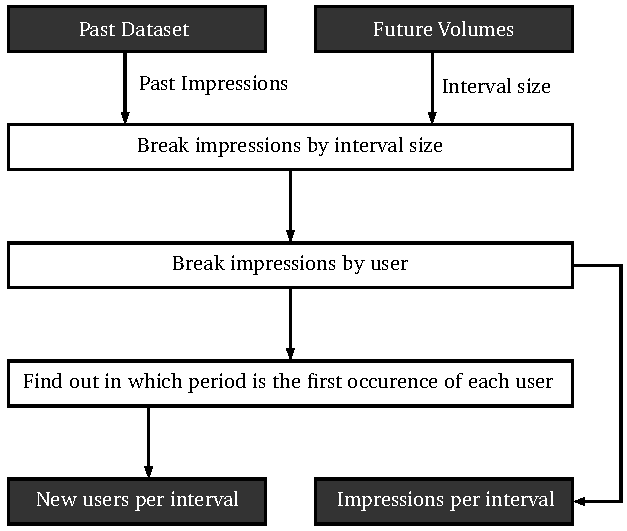
\includegraphics[]{pre_processing_i} \caption{ High level overview
of the Dataset Pre-processing} \label{fig:pre_processing_i} \end{center} \end{figure}

This phase (figure~\ref{fig:pre_processing_i}) can be considered the simpler phase of the whole approach. Its main
goal is to provide impressions organized by a defined time interval and 
place the first occurrence of each user in the correct interval, to better
organize data for the next phases.
\\

This is simply done by reading each line of the dataset and comparing with the
start date of the dataset placing it on the correct interval, also identify
which user is responsible for that impression and, if it is its first occurrence
, place it as a new user for the interval where the impression belong.

\subsubsection{Calculate Statistics (ii)}\label{subsubsec:stats}

\begin{figure}[h] \begin{center} \leavevmode
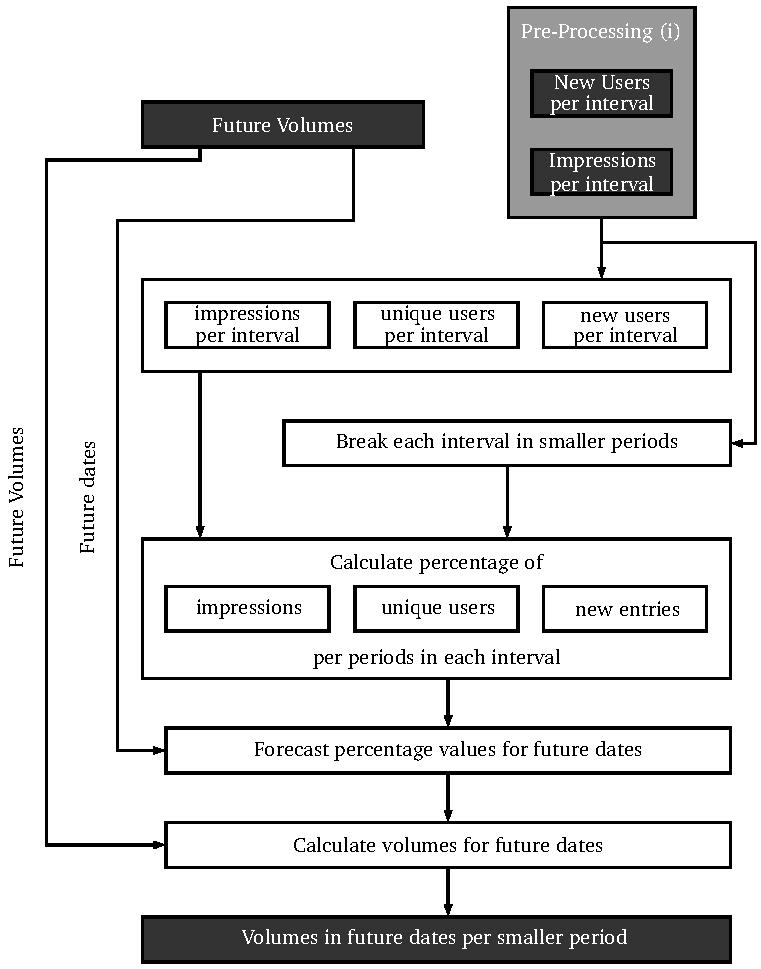
\includegraphics[]{calculate_stats} \caption{ High level overview
of statistics calculation} \label{fig:calculate_stats_ii} \end{center} \end{figure}

The main purpose of the sub-phase represented in the figure~\ref{fig:calculate_stats_ii} is
to distribute the volumes predict for a certain interval in smaller periods
based on historical distribution of the volumes for the same period.

In order to obtain better resolution of how the data is distributed on the
interval, these intervals are broken down in periods of one hour each. Now to
understand how the volumes of the interval are distributed through the time periods,
the data from the same interval up to two weeks before the interval which is
currently
being processed is used. For each hour period of historical interval the
percentage of the total volume is calculated.
To calculate the distribution , the input is the mean of the values from the
same interval, the week before, and two weeks before. If there is only one
previous week available, then the value of the current period is the same as the
value from the week before; if there are no previous weeks available, the
distribution of the interval volumes is done by dividing uniformly by each hour
period.
After the percentages are
calculated, they are multiplied by the total volumes to obtain the absolute
values for each interval.
\\
For each hour period the following values are calculated:
\begin{itemize}
  \item \textbf{Number of impressions}, this value represents how many requests
    were done during that space in time;
  \item \textbf{Number of users}, number of different users present during that
    space in time;
  \item \textbf{Number of first occurence users}, number of different users that
    occur for the first time in the interval during that specific hour period;
  \item \textbf{Number of new users}, number of different users that are
    completely new to the dataset and occur for the first time in that specific
    hour period.
\end{itemize}

In order to be valid, these variables have to respect these constraints:
\begin{itemize}
\item the number of impressions must be equal or greater than the number of
  users for a specific period;
\item the number of users must be less or equal to the sum of number of first
  occurrence users;
\item the number of new users and number of users that appear on the one hour
periods prior to this period that belong to the same interval;
\item the number of first occurrence users plus the number of new users must be
  equal or less than the number of users for the time period.
\end{itemize}

To guarantee the integrity of the result, these conditions have to be verified.
So, after the results for every hour period of a certain interval of time are
calculated, a constraint check is performed and the results are adjusted
accordingly. 
And to do so the approach implemented on
algorithm~\ref{alg:adjust_values} can be used to fulfil this task.
\\

\begin{algorithm}[H]
  \LinesNumbered
  \SetNlSty{texttt}{(}{)}
  \KwData{$periods$, a list of one tuple for each period; $volumes$,
  a tuple containing the expected values for the interval}
  \KwResult{A list of one tuple for each period, containing the adjusted values
  to meet the imposed constraints}
  \BlankLine

  \While{the sum tuples for all periods != $volumes$}{
    $diff$ = $volumes$ - $sum(periods)$\;
    \For{each element of $periods$}{
      To each constraint not respected, change the value according to the rule and
      then add the difference to the respective $diff$\;
      \If{any constraint not violated and the respective value of $diff$ is not
      0}{ 
        change the respective value while still respect the imposed constraint\;
      }
    }
}
  \BlankLine
  \vspace{0.5cm}
  \caption[Constraint adjustement for statistics]{
    Values adjustment to meet the imposed constraints algorithm
  }
  \label{alg:adjust_values} \end{algorithm}

At the end of this phase we have calculated all the four
values for every future interval for which we want to predict the impressions.


\subsubsection{Fill Future Data (iii)}\label{subsubsec:fill_data}

\begin{figure}[h] \begin{center} \leavevmode
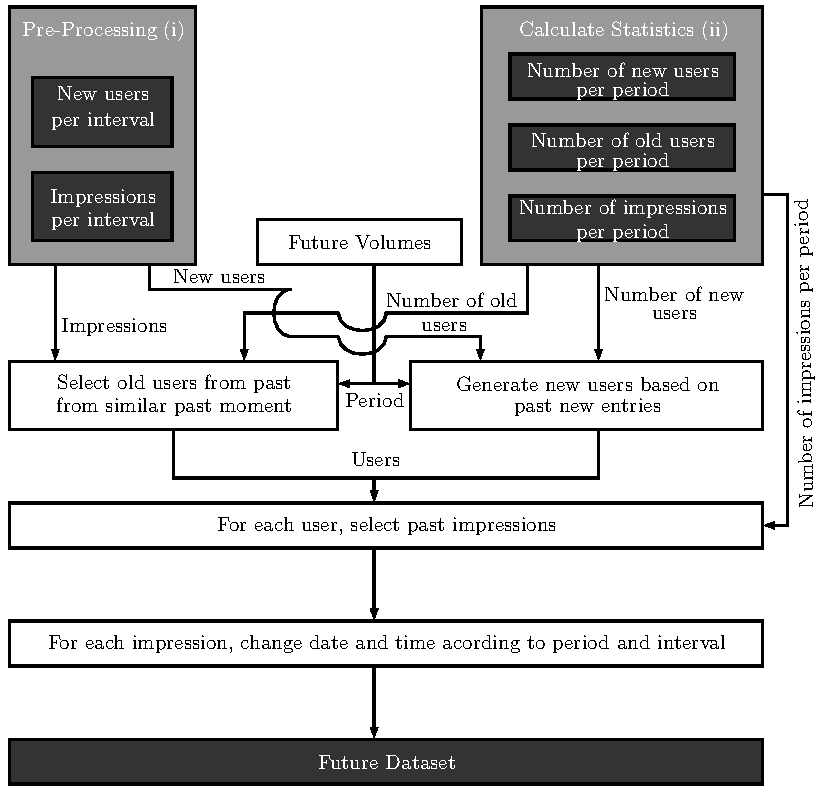
\includegraphics[]{fill_future} \caption{ High level overview
of fill future data} \label{fig:fill_future_iii} \end{center} \end{figure}

The last sub-phase of the dataset generation phase is responsible for selecting
which users and impressions, from the dataset that represents past activity,
that will reappear in the future with some changes.

To be able to capture the correct characteristics, so that the future follows the
trends of the past, the first step must be the selecting of the relevant periods of
time in the past that are equivalent to the one which is currently being filled.
This approach uses the same period from previous weeks ranked by proximity to
the date, which makes more likely to use users from the previous week than two
weeks ago.

After the correct dates are found, the users that will reappear in a given
period must be selected taking into account the limits imposed by the volumes
predicted on the previous sub-phase (\ref{subsubsec:stats}).

The process of the selection of old users is non-deterministic (uses random generated
values to select which past users will reappear), but assures that does not enter
an infinite loop, by terminating if it spends more than a $threshold$ of cycles
without getting a valid result. This is done in reverse chronological order,
where we first select users from the week before. If there are not enough
users we use data from previous weeks.

To complete the process of selection of users that will appear in the given
period, we need to ''generate'' new users. Since we have no knowledge of the
data that represents an impression other than it has a date and an user
identification token, this process is more a selection, than a generation, of
past users that occurred for the first time on similar periods of the past, and
then their date and user identification are changed according to the period for
where this user will reappear. Like the previous selection process, this one also
takes into account the chronological distance between events. First we use new
occurrences from same period, starting on the previous week until the first date
of the past dataset (if there are not enough users available users from the
same interval\footnote{Note that an interval is composed by multiple one hour
periods.} are used, if more users are needed then users from any interval of the
dataset are used).

To complete the process of filling the future impressions, we still needed to
select which past impressions from the selected users will be used, and modify
them according to the period that is being computed. First we randomly
select one impression from each user, since all the selected users must appear at
least one time. Afterwards, all the impressions are sorted in a random order, and
the impressions are selected randomly one by one until the requirements are
fulfilled.
The selection process takes into account the number of impressions associated
with a user; a user with many impressions in the past has more chances for one
of his impressions to be selected.
After all impressions are select, their time value is updated to a random time
inside the current time interval.

These steps must be executed for each period that we want to predict.

At the end we have a complete dataset that represent the volumes predicted on
the Volume Forecasting phase (\ref{subsec:volume_forecast}), which are ready to be used on a simulator.

\section{Experimental Setup}

\subsection{Dataset format}

To develop this approach a dataset containing the time of the occurrence, user
id token, and other information, like the browser, location, cookies, etc. was
used, an example of this dataset in on the table~\ref{tab:dataset}.

\begin{table}[h]
\tiny
\begin{tabular}{lllll}
\multicolumn{1}{l|}{\textbf{Time}}                    & \multicolumn{1}{l|}{\textbf{UserId}}                      & \multicolumn{1}{l|}{\textbf{AdvertiserId}}     & \multicolumn{1}{l|}{\textbf{OrderId}}  & \textbf{LineItemId}         \\ \hline
\multicolumn{1}{l|}{2013-11-26-00:00:01}              & \multicolumn{1}{l|}{89e3b953-4422-49cb-bc10-8e869b30f0ab} & \multicolumn{1}{l|}{26621901}                  & \multicolumn{1}{l|}{138907941}         & 107293701                   \\
                                                      &                                                           &                                                &                                        &                             \\
\multicolumn{1}{l|}{\textbf{CreativeId}}              & \multicolumn{1}{l|}{\textbf{CreativeVersion}}             & \multicolumn{1}{l|}{\textbf{CreativeSize}}     & \multicolumn{1}{l|}{\textbf{AdUnitId}} & \textbf{CustomTargeting}    \\ \hline
\multicolumn{1}{l|}{32278541781}                      & \multicolumn{1}{l|}{1}                                    & \multicolumn{1}{l|}{1x2}                       & \multicolumn{1}{l|}{27191421}          & pos=0;showroom=ab           \\
                                                      &                                                           &                                                &                                        &                             \\
\multicolumn{1}{l|}{\textbf{Domain}}                  & \multicolumn{1}{l|}{\textbf{CountryId}}                   & \multicolumn{1}{l|}{\textbf{Country}}          & \multicolumn{1}{l|}{\textbf{RegionId}} & \textbf{Region}             \\ \hline
\multicolumn{1}{l|}{2e07dc054c5bdcec109605689ec8e11f} & \multicolumn{1}{l|}{2276}                                 & \multicolumn{1}{l|}{Germany}                   & \multicolumn{1}{l|}{20240}             & Saxony-Anhalt               \\
                                                      &                                                           &                                                &                                        &                             \\
\multicolumn{1}{l|}{\textbf{CityId}}                  & \multicolumn{1}{l|}{\textbf{City}}                        & \multicolumn{1}{l|}{\textbf{BrowserId}}        & \multicolumn{1}{l|}{\textbf{Browser}}  & \textbf{OSId}               \\ \hline
\multicolumn{1}{l|}{1004957}                          & \multicolumn{1}{l|}{Hettstedt}                            & \multicolumn{1}{l|}{500072}                    & \multicolumn{1}{l|}{Google Chrome}     & 501011                      \\
                                                      &                                                           &                                                &                                        &                             \\
\multicolumn{1}{l|}{\textbf{OS}}                      & \multicolumn{1}{l|}{\textbf{OSVersion}}                   & \multicolumn{1}{l|}{\textbf{BandWidth}}        & \multicolumn{1}{l|}{\textbf{TimeUsec}} & \textbf{AudienceSegmentIds} \\ \hline
\multicolumn{1}{l|}{Microsoft Windows 7}              & \multicolumn{1}{l|}{}                                     & \multicolumn{1}{l|}{adsl-8mbps}                & \multicolumn{1}{l|}{1384817822}        &                             \\
                                                      &                                                           &                                                &                                        &                             \\
\multicolumn{1}{l|}{\textbf{Product}}                 & \multicolumn{1}{l|}{\textbf{RequestedAdUnitSizes}}        & \multicolumn{1}{l|}{\textbf{BandwidthGroupId}} &                                        &                             \\ \cline{1-3}
\multicolumn{1}{l|}{Ad Server}                        & \multicolumn{1}{l|}{1x2}                                  & \multicolumn{1}{l|}{3}                         &                                        &                            
\end{tabular}
\caption{Example data from the dataset used with the respective label}\label{tab:dataset}
\end{table}

The only fields that the solution depends on are the time and the user id token,
all the other fields are optional and the approach described above does not have
any specific knowledge about them, nor it depends of it. The optional parameters
can be useful on the segmentation phase, to divide the dataset in smaller
datasets in order to capture more specific characteristics.

The design decision of not using anything besides the time and user id, was made
because the proposed solution should be agnostic of the data that it analyses.
Mostly because the data available is not standardised, and the solution should be
able to be used on data from multiple sources, with each source having its own
way of saving activities.

\subsection{Experimental Setup configurations}

In order to be able to test the previously described approach, it was
implemented
using $Python$ . The experimental setup is completely modular, with every phase
being
totally independent of the other and the data that any phase process can come
from other sources other than the implemented ones.
Other than $Python$, $R$ was used in order to use the $ARIMA$ model.

\subsubsection*{Segmentation}

In this phase there are two implement methods, as explained
before on ~\ref{subsec:seg}. The $data stream-based$ algorithm does not have any
configuration parameters, so every test done was executed using the same parameters.
On the other hand for the segmentation by parameters, the parameters to be used for
the division can be changed, so different configurations were tested.

This phase cannot be directly validated nor compared, so the results were
only validated and compared after the forecast phase.

\subsubsection*{Volume Forecast}

On this phase, the $ARIMA$ model is used to predict the behaviour of the time
series for the time interval where we want to predict the volume values. To use
the $ARIMA$ model, the function $auto.arima$ the package $forecast$ \cite{hyndman2007automatic} for $R$
was used, using a $Python$ wrapper in order to process the data. The $R$ is only
responsible for the prediction.

The function used allows the configuration of various parameters, most of which
were covered by the tests (for example, the usage of \emph{drift terms}).
The frequency of the time series object in
$R$ is also configurable.

Different time intervals were also tested, in order to understand which interval
produces better results.

To compare these results, $RMSE$ and $MASE$ where used.

\subsubsection*{Dataset Generation}

This last phase does not take any additional parameters. It uses the values
that had been forecast in the volume forecast phase and the old dataset in order to build
a dataset which represents the future.

This phase was tested using synthetic generated past datasets which contained certain
changes in some parameters (examples being changes in browser usage and addition of new domains)

???SIMULATOR???

\section{Conclusion}

As mentioned before, this process has multiple phases where it tries to capture the
maximum amount of information about the past in order to more accurately predict
the future.
This chapter ends with an high level overview of the experimental setup, for which
the results will be presented and analysed on the next chapter.


\chapter{Conclusions and Future Work} \label{chap:concl}

\section*{}

\section{Objectives Fulfilment}

We proposed the used of the three phase approach (Chapter~\ref{chap:chap4}) in
order to obtain a more rich future prediction of the web activity on a network.
The first phase allow to obtain better prediction for certain characteristics,
the second phase allow to predict their volumes in the future, lastly the third
phase fill the future data with additional information from the past while follow
the tends of the predicted volumes.

Our results show that the usage of dataset segmentation allow to get moderate to
good improvements while predicting the volumes.

At the end we get a dataset with the same format as the inputed, but with future
data following the main characteristics of the past while amplifying some of the
more important characteristics for the future.

This dataset completely ready to be used on simulations of online advertising
campaigns in order to perceive their behaviour in the future.

\section{Future Work}

In order, to achieve better results some other approaches could be explored. For
example, use $MLP$, multilayer perceptron to predict the time series values
instead of the $ARIMA$.

It would also make sense to explore the usage of additional time series for new
entries of each parameter in order to correctly predict the occurrence of a new
website, for example. This phase will also need an additional knowledge about
some of the parameters to get better results, for example know how to generate a
new domain. This knowledge should be optional in order to maintain the data
agnostic approach, but when available probably would improve the results.

Another road to be explored is segmentation phase for example the usage
recursive parameter segmentation. For example, segment the whole dataset by
browser and then by country. It is my believe that this approach would get good
results if a huge volume of data were available.

It would also be interesting to test the resultant datasets on a real online
advertising campaign simulator in order to better assess the results in practical
applications.

 

%%----------------------------------------
%% Final materials
%%----------------------------------------

%% Bibliography
%% Comment the next command if BibTeX file not used
%% bibliography is in ``myrefs.bib''
\PrintBib{myrefs}

%% comment next 2 commands if numbered appendices are not used
%\appendix
%\chapter{Loren Ipsum} \label{ap1:loren}

Depois das conclusões e antes das referências bibliográficas,
apresenta-se neste anexo numerado o texto usado para preencher a
dissertação.

\section{O que é o \emph{Loren Ipsum}?}

\emph{\textbf{Lorem Ipsum}} is simply dummy text of the printing and
typesetting industry. Lorem Ipsum has been the industry's standard
dummy text ever since the 1500s, when an unknown printer took a galley
of type and scrambled it to make a type specimen book. It has survived
not only five centuries, but also the leap into electronic
typesetting, remaining essentially unchanged. It was popularised in
the 1960s with the release of Letraset sheets containing Lorem Ipsum
passages, and more recently with desktop publishing software like
Aldus PageMaker including versions of Lorem Ipsum~\citep{kn:Lip08}. 

\section{De onde Vem o Loren?}

Contrary to popular belief, Lorem Ipsum is not simply random text. It
has roots in a piece of classical Latin literature from 45 BC, making
it over 2000 years old. Richard McClintock, a Latin professor at
Hampden-Sydney College in Virginia, looked up one of the more obscure
Latin words, consectetur, from a Lorem Ipsum passage, and going
through the cites of the word in classical literature, discovered the
undoubtable source. Lorem Ipsum comes from sections 1.10.32 and
1.10.33 of ``de Finibus Bonorum et Malorum'' (The Extremes of Good and
Evil) by Cicero, written in 45 BC. This book is a treatise on the
theory of ethics, very popular during the Renaissance. The first line
of Lorem Ipsum, ``Lorem ipsum dolor sit amet\ldots'', comes from a line in
section 1.10.32.

The standard chunk of Lorem Ipsum used since the 1500s is reproduced
below for those interested. Sections 1.10.32 and 1.10.33 from ``de
Finibus Bonorum et Malorum'' by Cicero are also reproduced in their
exact original form, accompanied by English versions from the 1914
translation by H. Rackham.

\section{Porque se usa o Loren?}

It is a long established fact that a reader will be distracted by the
readable content of a page when looking at its layout. The point of
using Lorem Ipsum is that it has a more-or-less normal distribution of
letters, as opposed to using ``Content here, content here'', making it
look like readable English. Many desktop publishing packages and web
page editors now use Lorem Ipsum as their default model text, and a
search for ``lorem ipsum'' will uncover many web sites still in their
infancy. Various versions have evolved over the years, sometimes by
accident, sometimes on purpose (injected humour and the like). 

\section{Onde se Podem Encontrar Exemplos?}

There are many variations of passages of Lorem Ipsum available, but
the majority have suffered alteration in some form, by injected
humour, or randomised words which don't look even slightly
believable. If you are going to use a passage of Lorem Ipsum, you need
to be sure there isn't anything embarrassing hidden in the middle of
text. All the Lorem Ipsum generators on the Internet tend to repeat
predefined chunks as necessary, making this the first true generator
on the Internet. It uses a dictionary of over 200 Latin words,
combined with a handful of model sentence structures, to generate
Lorem Ipsum which looks reasonable. The generated Lorem Ipsum is
therefore always free from repetition, injected humour, or
non-characteristic words etc. 


%% Index
%% Uncomment next command if index is required
%% don't forget to run ``makeindex mieic-en'' command
%\PrintIndex

\end{document}
